\documentclass[11pt]{article}

    \usepackage[breakable]{tcolorbox}
    \usepackage{parskip} % Stop auto-indenting (to mimic markdown behaviour)
    

    % Basic figure setup, for now with no caption control since it's done
    % automatically by Pandoc (which extracts ![](path) syntax from Markdown).
    \usepackage{graphicx}
    % Maintain compatibility with old templates. Remove in nbconvert 6.0
    \let\Oldincludegraphics\includegraphics
    % Ensure that by default, figures have no caption (until we provide a
    % proper Figure object with a Caption API and a way to capture that
    % in the conversion process - todo).
    \usepackage{caption}
    \DeclareCaptionFormat{nocaption}{}
    \captionsetup{format=nocaption,aboveskip=0pt,belowskip=0pt}

    \usepackage{float}
    \floatplacement{figure}{H} % forces figures to be placed at the correct location
    \usepackage{xcolor} % Allow colors to be defined
    \usepackage{enumerate} % Needed for markdown enumerations to work
    \usepackage{geometry} % Used to adjust the document margins
    \usepackage{amsmath} % Equations
    \usepackage{amssymb} % Equations
    \usepackage{textcomp} % defines textquotesingle
    % Hack from http://tex.stackexchange.com/a/47451/13684:
    \AtBeginDocument{%
        \def\PYZsq{\textquotesingle}% Upright quotes in Pygmentized code
    }
    \usepackage{upquote} % Upright quotes for verbatim code
    \usepackage{eurosym} % defines \euro

    \usepackage{iftex}
    \ifPDFTeX
        \usepackage[T1]{fontenc}
        \IfFileExists{alphabeta.sty}{
              \usepackage{alphabeta}
          }{
              \usepackage[mathletters]{ucs}
              \usepackage[utf8x]{inputenc}
          }
    \else
        \usepackage{fontspec}
        \usepackage{unicode-math}
    \fi

    \usepackage{fancyvrb} % verbatim replacement that allows latex
    \usepackage{grffile} % extends the file name processing of package graphics
                         % to support a larger range
    \makeatletter % fix for old versions of grffile with XeLaTeX
    \@ifpackagelater{grffile}{2019/11/01}
    {
      % Do nothing on new versions
    }
    {
      \def\Gread@@xetex#1{%
        \IfFileExists{"\Gin@base".bb}%
        {\Gread@eps{\Gin@base.bb}}%
        {\Gread@@xetex@aux#1}%
      }
    }
    \makeatother
    \usepackage[Export]{adjustbox} % Used to constrain images to a maximum size
    \adjustboxset{max size={0.9\linewidth}{0.9\paperheight}}

    % The hyperref package gives us a pdf with properly built
    % internal navigation ('pdf bookmarks' for the table of contents,
    % internal cross-reference links, web links for URLs, etc.)
    \usepackage{hyperref}
    % The default LaTeX title has an obnoxious amount of whitespace. By default,
    % titling removes some of it. It also provides customization options.
    \usepackage{titling}
    \usepackage{longtable} % longtable support required by pandoc >1.10
    \usepackage{booktabs}  % table support for pandoc > 1.12.2
    \usepackage{array}     % table support for pandoc >= 2.11.3
    \usepackage{calc}      % table minipage width calculation for pandoc >= 2.11.1
    \usepackage[inline]{enumitem} % IRkernel/repr support (it uses the enumerate* environment)
    \usepackage[normalem]{ulem} % ulem is needed to support strikethroughs (\sout)
                                % normalem makes italics be italics, not underlines
    \usepackage{soul}      % strikethrough (\st) support for pandoc >= 3.0.0
    \usepackage{mathrsfs}
    

    
    % Colors for the hyperref package
    \definecolor{urlcolor}{rgb}{0,.145,.698}
    \definecolor{linkcolor}{rgb}{.71,0.21,0.01}
    \definecolor{citecolor}{rgb}{.12,.54,.11}

    % ANSI colors
    \definecolor{ansi-black}{HTML}{3E424D}
    \definecolor{ansi-black-intense}{HTML}{282C36}
    \definecolor{ansi-red}{HTML}{E75C58}
    \definecolor{ansi-red-intense}{HTML}{B22B31}
    \definecolor{ansi-green}{HTML}{00A250}
    \definecolor{ansi-green-intense}{HTML}{007427}
    \definecolor{ansi-yellow}{HTML}{DDB62B}
    \definecolor{ansi-yellow-intense}{HTML}{B27D12}
    \definecolor{ansi-blue}{HTML}{208FFB}
    \definecolor{ansi-blue-intense}{HTML}{0065CA}
    \definecolor{ansi-magenta}{HTML}{D160C4}
    \definecolor{ansi-magenta-intense}{HTML}{A03196}
    \definecolor{ansi-cyan}{HTML}{60C6C8}
    \definecolor{ansi-cyan-intense}{HTML}{258F8F}
    \definecolor{ansi-white}{HTML}{C5C1B4}
    \definecolor{ansi-white-intense}{HTML}{A1A6B2}
    \definecolor{ansi-default-inverse-fg}{HTML}{FFFFFF}
    \definecolor{ansi-default-inverse-bg}{HTML}{000000}

    % common color for the border for error outputs.
    \definecolor{outerrorbackground}{HTML}{FFDFDF}

    % commands and environments needed by pandoc snippets
    % extracted from the output of `pandoc -s`
    \providecommand{\tightlist}{%
      \setlength{\itemsep}{0pt}\setlength{\parskip}{0pt}}
    \DefineVerbatimEnvironment{Highlighting}{Verbatim}{commandchars=\\\{\}}
    % Add ',fontsize=\small' for more characters per line
    \newenvironment{Shaded}{}{}
    \newcommand{\KeywordTok}[1]{\textcolor[rgb]{0.00,0.44,0.13}{\textbf{{#1}}}}
    \newcommand{\DataTypeTok}[1]{\textcolor[rgb]{0.56,0.13,0.00}{{#1}}}
    \newcommand{\DecValTok}[1]{\textcolor[rgb]{0.25,0.63,0.44}{{#1}}}
    \newcommand{\BaseNTok}[1]{\textcolor[rgb]{0.25,0.63,0.44}{{#1}}}
    \newcommand{\FloatTok}[1]{\textcolor[rgb]{0.25,0.63,0.44}{{#1}}}
    \newcommand{\CharTok}[1]{\textcolor[rgb]{0.25,0.44,0.63}{{#1}}}
    \newcommand{\StringTok}[1]{\textcolor[rgb]{0.25,0.44,0.63}{{#1}}}
    \newcommand{\CommentTok}[1]{\textcolor[rgb]{0.38,0.63,0.69}{\textit{{#1}}}}
    \newcommand{\OtherTok}[1]{\textcolor[rgb]{0.00,0.44,0.13}{{#1}}}
    \newcommand{\AlertTok}[1]{\textcolor[rgb]{1.00,0.00,0.00}{\textbf{{#1}}}}
    \newcommand{\FunctionTok}[1]{\textcolor[rgb]{0.02,0.16,0.49}{{#1}}}
    \newcommand{\RegionMarkerTok}[1]{{#1}}
    \newcommand{\ErrorTok}[1]{\textcolor[rgb]{1.00,0.00,0.00}{\textbf{{#1}}}}
    \newcommand{\NormalTok}[1]{{#1}}

    % Additional commands for more recent versions of Pandoc
    \newcommand{\ConstantTok}[1]{\textcolor[rgb]{0.53,0.00,0.00}{{#1}}}
    \newcommand{\SpecialCharTok}[1]{\textcolor[rgb]{0.25,0.44,0.63}{{#1}}}
    \newcommand{\VerbatimStringTok}[1]{\textcolor[rgb]{0.25,0.44,0.63}{{#1}}}
    \newcommand{\SpecialStringTok}[1]{\textcolor[rgb]{0.73,0.40,0.53}{{#1}}}
    \newcommand{\ImportTok}[1]{{#1}}
    \newcommand{\DocumentationTok}[1]{\textcolor[rgb]{0.73,0.13,0.13}{\textit{{#1}}}}
    \newcommand{\AnnotationTok}[1]{\textcolor[rgb]{0.38,0.63,0.69}{\textbf{\textit{{#1}}}}}
    \newcommand{\CommentVarTok}[1]{\textcolor[rgb]{0.38,0.63,0.69}{\textbf{\textit{{#1}}}}}
    \newcommand{\VariableTok}[1]{\textcolor[rgb]{0.10,0.09,0.49}{{#1}}}
    \newcommand{\ControlFlowTok}[1]{\textcolor[rgb]{0.00,0.44,0.13}{\textbf{{#1}}}}
    \newcommand{\OperatorTok}[1]{\textcolor[rgb]{0.40,0.40,0.40}{{#1}}}
    \newcommand{\BuiltInTok}[1]{{#1}}
    \newcommand{\ExtensionTok}[1]{{#1}}
    \newcommand{\PreprocessorTok}[1]{\textcolor[rgb]{0.74,0.48,0.00}{{#1}}}
    \newcommand{\AttributeTok}[1]{\textcolor[rgb]{0.49,0.56,0.16}{{#1}}}
    \newcommand{\InformationTok}[1]{\textcolor[rgb]{0.38,0.63,0.69}{\textbf{\textit{{#1}}}}}
    \newcommand{\WarningTok}[1]{\textcolor[rgb]{0.38,0.63,0.69}{\textbf{\textit{{#1}}}}}


    % Define a nice break command that doesn't care if a line doesn't already
    % exist.
    \def\br{\hspace*{\fill} \\* }
    % Math Jax compatibility definitions
    \def\gt{>}
    \def\lt{<}
    \let\Oldtex\TeX
    \let\Oldlatex\LaTeX
    \renewcommand{\TeX}{\textrm{\Oldtex}}
    \renewcommand{\LaTeX}{\textrm{\Oldlatex}}
    % Document parameters
    % Document title
    \title{Module5-HW}
    
    
    
    
    
    
    
% Pygments definitions
\makeatletter
\def\PY@reset{\let\PY@it=\relax \let\PY@bf=\relax%
    \let\PY@ul=\relax \let\PY@tc=\relax%
    \let\PY@bc=\relax \let\PY@ff=\relax}
\def\PY@tok#1{\csname PY@tok@#1\endcsname}
\def\PY@toks#1+{\ifx\relax#1\empty\else%
    \PY@tok{#1}\expandafter\PY@toks\fi}
\def\PY@do#1{\PY@bc{\PY@tc{\PY@ul{%
    \PY@it{\PY@bf{\PY@ff{#1}}}}}}}
\def\PY#1#2{\PY@reset\PY@toks#1+\relax+\PY@do{#2}}

\@namedef{PY@tok@w}{\def\PY@tc##1{\textcolor[rgb]{0.73,0.73,0.73}{##1}}}
\@namedef{PY@tok@c}{\let\PY@it=\textit\def\PY@tc##1{\textcolor[rgb]{0.24,0.48,0.48}{##1}}}
\@namedef{PY@tok@cp}{\def\PY@tc##1{\textcolor[rgb]{0.61,0.40,0.00}{##1}}}
\@namedef{PY@tok@k}{\let\PY@bf=\textbf\def\PY@tc##1{\textcolor[rgb]{0.00,0.50,0.00}{##1}}}
\@namedef{PY@tok@kp}{\def\PY@tc##1{\textcolor[rgb]{0.00,0.50,0.00}{##1}}}
\@namedef{PY@tok@kt}{\def\PY@tc##1{\textcolor[rgb]{0.69,0.00,0.25}{##1}}}
\@namedef{PY@tok@o}{\def\PY@tc##1{\textcolor[rgb]{0.40,0.40,0.40}{##1}}}
\@namedef{PY@tok@ow}{\let\PY@bf=\textbf\def\PY@tc##1{\textcolor[rgb]{0.67,0.13,1.00}{##1}}}
\@namedef{PY@tok@nb}{\def\PY@tc##1{\textcolor[rgb]{0.00,0.50,0.00}{##1}}}
\@namedef{PY@tok@nf}{\def\PY@tc##1{\textcolor[rgb]{0.00,0.00,1.00}{##1}}}
\@namedef{PY@tok@nc}{\let\PY@bf=\textbf\def\PY@tc##1{\textcolor[rgb]{0.00,0.00,1.00}{##1}}}
\@namedef{PY@tok@nn}{\let\PY@bf=\textbf\def\PY@tc##1{\textcolor[rgb]{0.00,0.00,1.00}{##1}}}
\@namedef{PY@tok@ne}{\let\PY@bf=\textbf\def\PY@tc##1{\textcolor[rgb]{0.80,0.25,0.22}{##1}}}
\@namedef{PY@tok@nv}{\def\PY@tc##1{\textcolor[rgb]{0.10,0.09,0.49}{##1}}}
\@namedef{PY@tok@no}{\def\PY@tc##1{\textcolor[rgb]{0.53,0.00,0.00}{##1}}}
\@namedef{PY@tok@nl}{\def\PY@tc##1{\textcolor[rgb]{0.46,0.46,0.00}{##1}}}
\@namedef{PY@tok@ni}{\let\PY@bf=\textbf\def\PY@tc##1{\textcolor[rgb]{0.44,0.44,0.44}{##1}}}
\@namedef{PY@tok@na}{\def\PY@tc##1{\textcolor[rgb]{0.41,0.47,0.13}{##1}}}
\@namedef{PY@tok@nt}{\let\PY@bf=\textbf\def\PY@tc##1{\textcolor[rgb]{0.00,0.50,0.00}{##1}}}
\@namedef{PY@tok@nd}{\def\PY@tc##1{\textcolor[rgb]{0.67,0.13,1.00}{##1}}}
\@namedef{PY@tok@s}{\def\PY@tc##1{\textcolor[rgb]{0.73,0.13,0.13}{##1}}}
\@namedef{PY@tok@sd}{\let\PY@it=\textit\def\PY@tc##1{\textcolor[rgb]{0.73,0.13,0.13}{##1}}}
\@namedef{PY@tok@si}{\let\PY@bf=\textbf\def\PY@tc##1{\textcolor[rgb]{0.64,0.35,0.47}{##1}}}
\@namedef{PY@tok@se}{\let\PY@bf=\textbf\def\PY@tc##1{\textcolor[rgb]{0.67,0.36,0.12}{##1}}}
\@namedef{PY@tok@sr}{\def\PY@tc##1{\textcolor[rgb]{0.64,0.35,0.47}{##1}}}
\@namedef{PY@tok@ss}{\def\PY@tc##1{\textcolor[rgb]{0.10,0.09,0.49}{##1}}}
\@namedef{PY@tok@sx}{\def\PY@tc##1{\textcolor[rgb]{0.00,0.50,0.00}{##1}}}
\@namedef{PY@tok@m}{\def\PY@tc##1{\textcolor[rgb]{0.40,0.40,0.40}{##1}}}
\@namedef{PY@tok@gh}{\let\PY@bf=\textbf\def\PY@tc##1{\textcolor[rgb]{0.00,0.00,0.50}{##1}}}
\@namedef{PY@tok@gu}{\let\PY@bf=\textbf\def\PY@tc##1{\textcolor[rgb]{0.50,0.00,0.50}{##1}}}
\@namedef{PY@tok@gd}{\def\PY@tc##1{\textcolor[rgb]{0.63,0.00,0.00}{##1}}}
\@namedef{PY@tok@gi}{\def\PY@tc##1{\textcolor[rgb]{0.00,0.52,0.00}{##1}}}
\@namedef{PY@tok@gr}{\def\PY@tc##1{\textcolor[rgb]{0.89,0.00,0.00}{##1}}}
\@namedef{PY@tok@ge}{\let\PY@it=\textit}
\@namedef{PY@tok@gs}{\let\PY@bf=\textbf}
\@namedef{PY@tok@gp}{\let\PY@bf=\textbf\def\PY@tc##1{\textcolor[rgb]{0.00,0.00,0.50}{##1}}}
\@namedef{PY@tok@go}{\def\PY@tc##1{\textcolor[rgb]{0.44,0.44,0.44}{##1}}}
\@namedef{PY@tok@gt}{\def\PY@tc##1{\textcolor[rgb]{0.00,0.27,0.87}{##1}}}
\@namedef{PY@tok@err}{\def\PY@bc##1{{\setlength{\fboxsep}{\string -\fboxrule}\fcolorbox[rgb]{1.00,0.00,0.00}{1,1,1}{\strut ##1}}}}
\@namedef{PY@tok@kc}{\let\PY@bf=\textbf\def\PY@tc##1{\textcolor[rgb]{0.00,0.50,0.00}{##1}}}
\@namedef{PY@tok@kd}{\let\PY@bf=\textbf\def\PY@tc##1{\textcolor[rgb]{0.00,0.50,0.00}{##1}}}
\@namedef{PY@tok@kn}{\let\PY@bf=\textbf\def\PY@tc##1{\textcolor[rgb]{0.00,0.50,0.00}{##1}}}
\@namedef{PY@tok@kr}{\let\PY@bf=\textbf\def\PY@tc##1{\textcolor[rgb]{0.00,0.50,0.00}{##1}}}
\@namedef{PY@tok@bp}{\def\PY@tc##1{\textcolor[rgb]{0.00,0.50,0.00}{##1}}}
\@namedef{PY@tok@fm}{\def\PY@tc##1{\textcolor[rgb]{0.00,0.00,1.00}{##1}}}
\@namedef{PY@tok@vc}{\def\PY@tc##1{\textcolor[rgb]{0.10,0.09,0.49}{##1}}}
\@namedef{PY@tok@vg}{\def\PY@tc##1{\textcolor[rgb]{0.10,0.09,0.49}{##1}}}
\@namedef{PY@tok@vi}{\def\PY@tc##1{\textcolor[rgb]{0.10,0.09,0.49}{##1}}}
\@namedef{PY@tok@vm}{\def\PY@tc##1{\textcolor[rgb]{0.10,0.09,0.49}{##1}}}
\@namedef{PY@tok@sa}{\def\PY@tc##1{\textcolor[rgb]{0.73,0.13,0.13}{##1}}}
\@namedef{PY@tok@sb}{\def\PY@tc##1{\textcolor[rgb]{0.73,0.13,0.13}{##1}}}
\@namedef{PY@tok@sc}{\def\PY@tc##1{\textcolor[rgb]{0.73,0.13,0.13}{##1}}}
\@namedef{PY@tok@dl}{\def\PY@tc##1{\textcolor[rgb]{0.73,0.13,0.13}{##1}}}
\@namedef{PY@tok@s2}{\def\PY@tc##1{\textcolor[rgb]{0.73,0.13,0.13}{##1}}}
\@namedef{PY@tok@sh}{\def\PY@tc##1{\textcolor[rgb]{0.73,0.13,0.13}{##1}}}
\@namedef{PY@tok@s1}{\def\PY@tc##1{\textcolor[rgb]{0.73,0.13,0.13}{##1}}}
\@namedef{PY@tok@mb}{\def\PY@tc##1{\textcolor[rgb]{0.40,0.40,0.40}{##1}}}
\@namedef{PY@tok@mf}{\def\PY@tc##1{\textcolor[rgb]{0.40,0.40,0.40}{##1}}}
\@namedef{PY@tok@mh}{\def\PY@tc##1{\textcolor[rgb]{0.40,0.40,0.40}{##1}}}
\@namedef{PY@tok@mi}{\def\PY@tc##1{\textcolor[rgb]{0.40,0.40,0.40}{##1}}}
\@namedef{PY@tok@il}{\def\PY@tc##1{\textcolor[rgb]{0.40,0.40,0.40}{##1}}}
\@namedef{PY@tok@mo}{\def\PY@tc##1{\textcolor[rgb]{0.40,0.40,0.40}{##1}}}
\@namedef{PY@tok@ch}{\let\PY@it=\textit\def\PY@tc##1{\textcolor[rgb]{0.24,0.48,0.48}{##1}}}
\@namedef{PY@tok@cm}{\let\PY@it=\textit\def\PY@tc##1{\textcolor[rgb]{0.24,0.48,0.48}{##1}}}
\@namedef{PY@tok@cpf}{\let\PY@it=\textit\def\PY@tc##1{\textcolor[rgb]{0.24,0.48,0.48}{##1}}}
\@namedef{PY@tok@c1}{\let\PY@it=\textit\def\PY@tc##1{\textcolor[rgb]{0.24,0.48,0.48}{##1}}}
\@namedef{PY@tok@cs}{\let\PY@it=\textit\def\PY@tc##1{\textcolor[rgb]{0.24,0.48,0.48}{##1}}}

\def\PYZbs{\char`\\}
\def\PYZus{\char`\_}
\def\PYZob{\char`\{}
\def\PYZcb{\char`\}}
\def\PYZca{\char`\^}
\def\PYZam{\char`\&}
\def\PYZlt{\char`\<}
\def\PYZgt{\char`\>}
\def\PYZsh{\char`\#}
\def\PYZpc{\char`\%}
\def\PYZdl{\char`\$}
\def\PYZhy{\char`\-}
\def\PYZsq{\char`\'}
\def\PYZdq{\char`\"}
\def\PYZti{\char`\~}
% for compatibility with earlier versions
\def\PYZat{@}
\def\PYZlb{[}
\def\PYZrb{]}
\makeatother


    % For linebreaks inside Verbatim environment from package fancyvrb.
    \makeatletter
        \newbox\Wrappedcontinuationbox
        \newbox\Wrappedvisiblespacebox
        \newcommand*\Wrappedvisiblespace {\textcolor{red}{\textvisiblespace}}
        \newcommand*\Wrappedcontinuationsymbol {\textcolor{red}{\llap{\tiny$\m@th\hookrightarrow$}}}
        \newcommand*\Wrappedcontinuationindent {3ex }
        \newcommand*\Wrappedafterbreak {\kern\Wrappedcontinuationindent\copy\Wrappedcontinuationbox}
        % Take advantage of the already applied Pygments mark-up to insert
        % potential linebreaks for TeX processing.
        %        {, <, #, %, $, ' and ": go to next line.
        %        _, }, ^, &, >, - and ~: stay at end of broken line.
        % Use of \textquotesingle for straight quote.
        \newcommand*\Wrappedbreaksatspecials {%
            \def\PYGZus{\discretionary{\char`\_}{\Wrappedafterbreak}{\char`\_}}%
            \def\PYGZob{\discretionary{}{\Wrappedafterbreak\char`\{}{\char`\{}}%
            \def\PYGZcb{\discretionary{\char`\}}{\Wrappedafterbreak}{\char`\}}}%
            \def\PYGZca{\discretionary{\char`\^}{\Wrappedafterbreak}{\char`\^}}%
            \def\PYGZam{\discretionary{\char`\&}{\Wrappedafterbreak}{\char`\&}}%
            \def\PYGZlt{\discretionary{}{\Wrappedafterbreak\char`\<}{\char`\<}}%
            \def\PYGZgt{\discretionary{\char`\>}{\Wrappedafterbreak}{\char`\>}}%
            \def\PYGZsh{\discretionary{}{\Wrappedafterbreak\char`\#}{\char`\#}}%
            \def\PYGZpc{\discretionary{}{\Wrappedafterbreak\char`\%}{\char`\%}}%
            \def\PYGZdl{\discretionary{}{\Wrappedafterbreak\char`\$}{\char`\$}}%
            \def\PYGZhy{\discretionary{\char`\-}{\Wrappedafterbreak}{\char`\-}}%
            \def\PYGZsq{\discretionary{}{\Wrappedafterbreak\textquotesingle}{\textquotesingle}}%
            \def\PYGZdq{\discretionary{}{\Wrappedafterbreak\char`\"}{\char`\"}}%
            \def\PYGZti{\discretionary{\char`\~}{\Wrappedafterbreak}{\char`\~}}%
        }
        % Some characters . , ; ? ! / are not pygmentized.
        % This macro makes them "active" and they will insert potential linebreaks
        \newcommand*\Wrappedbreaksatpunct {%
            \lccode`\~`\.\lowercase{\def~}{\discretionary{\hbox{\char`\.}}{\Wrappedafterbreak}{\hbox{\char`\.}}}%
            \lccode`\~`\,\lowercase{\def~}{\discretionary{\hbox{\char`\,}}{\Wrappedafterbreak}{\hbox{\char`\,}}}%
            \lccode`\~`\;\lowercase{\def~}{\discretionary{\hbox{\char`\;}}{\Wrappedafterbreak}{\hbox{\char`\;}}}%
            \lccode`\~`\:\lowercase{\def~}{\discretionary{\hbox{\char`\:}}{\Wrappedafterbreak}{\hbox{\char`\:}}}%
            \lccode`\~`\?\lowercase{\def~}{\discretionary{\hbox{\char`\?}}{\Wrappedafterbreak}{\hbox{\char`\?}}}%
            \lccode`\~`\!\lowercase{\def~}{\discretionary{\hbox{\char`\!}}{\Wrappedafterbreak}{\hbox{\char`\!}}}%
            \lccode`\~`\/\lowercase{\def~}{\discretionary{\hbox{\char`\/}}{\Wrappedafterbreak}{\hbox{\char`\/}}}%
            \catcode`\.\active
            \catcode`\,\active
            \catcode`\;\active
            \catcode`\:\active
            \catcode`\?\active
            \catcode`\!\active
            \catcode`\/\active
            \lccode`\~`\~
        }
    \makeatother

    \let\OriginalVerbatim=\Verbatim
    \makeatletter
    \renewcommand{\Verbatim}[1][1]{%
        %\parskip\z@skip
        \sbox\Wrappedcontinuationbox {\Wrappedcontinuationsymbol}%
        \sbox\Wrappedvisiblespacebox {\FV@SetupFont\Wrappedvisiblespace}%
        \def\FancyVerbFormatLine ##1{\hsize\linewidth
            \vtop{\raggedright\hyphenpenalty\z@\exhyphenpenalty\z@
                \doublehyphendemerits\z@\finalhyphendemerits\z@
                \strut ##1\strut}%
        }%
        % If the linebreak is at a space, the latter will be displayed as visible
        % space at end of first line, and a continuation symbol starts next line.
        % Stretch/shrink are however usually zero for typewriter font.
        \def\FV@Space {%
            \nobreak\hskip\z@ plus\fontdimen3\font minus\fontdimen4\font
            \discretionary{\copy\Wrappedvisiblespacebox}{\Wrappedafterbreak}
            {\kern\fontdimen2\font}%
        }%

        % Allow breaks at special characters using \PYG... macros.
        \Wrappedbreaksatspecials
        % Breaks at punctuation characters . , ; ? ! and / need catcode=\active
        \OriginalVerbatim[#1,codes*=\Wrappedbreaksatpunct]%
    }
    \makeatother

    % Exact colors from NB
    \definecolor{incolor}{HTML}{303F9F}
    \definecolor{outcolor}{HTML}{D84315}
    \definecolor{cellborder}{HTML}{CFCFCF}
    \definecolor{cellbackground}{HTML}{F7F7F7}

    % prompt
    \makeatletter
    \newcommand{\boxspacing}{\kern\kvtcb@left@rule\kern\kvtcb@boxsep}
    \makeatother
    \newcommand{\prompt}[4]{
        {\ttfamily\llap{{\color{#2}[#3]:\hspace{3pt}#4}}\vspace{-\baselineskip}}
    }
    

    
    % Prevent overflowing lines due to hard-to-break entities
    \sloppy
    % Setup hyperref package
    \hypersetup{
      breaklinks=true,  % so long urls are correctly broken across lines
      colorlinks=true,
      urlcolor=urlcolor,
      linkcolor=linkcolor,
      citecolor=citecolor,
      }
    % Slightly bigger margins than the latex defaults
    
    \geometry{verbose,tmargin=1in,bmargin=1in,lmargin=1in,rmargin=1in}
    
    

\begin{document}
    
    \maketitle
    
    

    Problem1-LeetcodeQ704-Binary Search-Easy

Given an array of integers nums which is sorted in ascending order, and an integer target, write a function to search target in nums. If target exists, then return its index. Otherwise, return -1.

You must write an algorithm with O(log n) runtime complexity.

 

Example 1:

Input: nums = [-1,0,3,5,9,12], target = 9
Output: 4
Explanation: 9 exists in nums and its index is 4
Example 2:

Input: nums = [-1,0,3,5,9,12], target = 2
Output: -1
Explanation: 2 does not exist in nums so return -1
 

Constraints:

1 <= nums.length <= 104
-104 < nums[i], target < 104
All the integers in nums are unique.
nums is sorted in ascending order.
    \subsubsection{pseudocode}\label{pseudocode}

    \begin{tcolorbox}[breakable, size=fbox, boxrule=1pt, pad at break*=1mm,colback=cellbackground, colframe=cellborder]
\prompt{In}{incolor}{ }{\boxspacing}
\begin{Verbatim}[commandchars=\\\{\}]
\PY{n}{Define} \PY{l+m+mi}{2} \PY{n}{pointers}
 \PY{n}{left} \PY{o}{=} \PY{l+m+mi}{0}
 \PY{n}{right} \PY{o}{=} \PY{n}{length} \PY{n}{of} \PY{n}{nums} \PY{o}{\PYZhy{}} \PY{l+m+mi}{1}

\PY{k}{while} \PY{n}{left} \PY{o}{\PYZlt{}}\PY{o}{=} \PY{n}{right}\PY{p}{:}
\PY{n}{middle} \PY{o}{=} \PY{p}{(}\PY{n}{left} \PY{o}{+} \PY{n}{right}\PY{p}{)} \PY{o}{/}\PY{o}{/} \PY{l+m+mi}{2}

\PY{k}{if} \PY{n}{nums}\PY{p}{[}\PY{n}{middle}\PY{p}{]} \PY{o}{\PYZlt{}} \PY{n}{target}\PY{p}{:}
    \PY{n}{left} \PY{o}{=} \PY{n}{middle} \PY{o}{+} \PY{l+m+mi}{1}
\PY{k}{else} \PY{k}{if} \PY{n}{nums}\PY{p}{[}\PY{n}{middle}\PY{p}{]} \PY{o}{\PYZgt{}} \PY{n}{target}\PY{p}{:}
    \PY{n}{right} \PY{o}{=} \PY{n}{middle} \PY{o}{\PYZhy{}} \PY{l+m+mi}{1}
\PY{k}{else}\PY{p}{:}
    \PY{k}{return} \PY{n}{middle}
\end{Verbatim}
\end{tcolorbox}

    \subsubsection{Q704 code.py}\label{q704-code.py}

    \begin{tcolorbox}[breakable, size=fbox, boxrule=1pt, pad at break*=1mm,colback=cellbackground, colframe=cellborder]
\prompt{In}{incolor}{3}{\boxspacing}
\begin{Verbatim}[commandchars=\\\{\}]
\PY{k+kn}{from} \PY{n+nn}{typing} \PY{k+kn}{import} \PY{n}{List}

\PY{k}{class} \PY{n+nc}{Solution}\PY{p}{:}
    \PY{k}{def} \PY{n+nf}{search}\PY{p}{(}\PY{n+nb+bp}{self}\PY{p}{,} \PY{n}{nums}\PY{p}{:} \PY{n}{List}\PY{p}{[}\PY{n+nb}{int}\PY{p}{]}\PY{p}{,} \PY{n}{target}\PY{p}{:} \PY{n+nb}{int}\PY{p}{)} \PY{o}{\PYZhy{}}\PY{o}{\PYZgt{}} \PY{n+nb}{int}\PY{p}{:}
        \PY{n}{left}\PY{p}{,} \PY{n}{right} \PY{o}{=} \PY{l+m+mi}{0}\PY{p}{,} \PY{n+nb}{len}\PY{p}{(}\PY{n}{nums}\PY{p}{)} \PY{o}{\PYZhy{}} \PY{l+m+mi}{1}
        
        \PY{k}{while} \PY{n}{left} \PY{o}{\PYZlt{}}\PY{o}{=} \PY{n}{right}\PY{p}{:}
            \PY{n}{middle} \PY{o}{=} \PY{p}{(}\PY{n}{left} \PY{o}{+} \PY{n}{right}\PY{p}{)} \PY{o}{/}\PY{o}{/} \PY{l+m+mi}{2}

            \PY{k}{if} \PY{n}{nums}\PY{p}{[}\PY{n}{middle}\PY{p}{]} \PY{o}{\PYZlt{}} \PY{n}{target}\PY{p}{:}
                \PY{n}{left} \PY{o}{=} \PY{n}{middle} \PY{o}{+} \PY{l+m+mi}{1}
            \PY{k}{elif} \PY{n}{nums}\PY{p}{[}\PY{n}{middle}\PY{p}{]} \PY{o}{\PYZgt{}} \PY{n}{target}\PY{p}{:}
                \PY{n}{right} \PY{o}{=} \PY{n}{middle} \PY{o}{\PYZhy{}} \PY{l+m+mi}{1}
            \PY{k}{else}\PY{p}{:}
                \PY{k}{return} \PY{n}{middle}
        \PY{k}{return} \PY{o}{\PYZhy{}}\PY{l+m+mi}{1}

\PY{c+c1}{\PYZsh{} Test case}
\PY{n}{nums} \PY{o}{=} \PY{p}{[}\PY{o}{\PYZhy{}}\PY{l+m+mi}{1}\PY{p}{,} \PY{l+m+mi}{0}\PY{p}{,} \PY{l+m+mi}{3}\PY{p}{,} \PY{l+m+mi}{5}\PY{p}{,} \PY{l+m+mi}{9}\PY{p}{,} \PY{l+m+mi}{12}\PY{p}{]}
\PY{n}{target} \PY{o}{=} \PY{l+m+mi}{9}
\PY{n}{solution} \PY{o}{=} \PY{n}{Solution}\PY{p}{(}\PY{p}{)}
\PY{n}{output} \PY{o}{=} \PY{n}{solution}\PY{o}{.}\PY{n}{search}\PY{p}{(}\PY{n}{nums}\PY{p}{,} \PY{n}{target}\PY{p}{)}
\PY{n+nb}{print}\PY{p}{(}\PY{l+s+sa}{f}\PY{l+s+s1}{\PYZsq{}}\PY{l+s+s1}{Input: nums = }\PY{l+s+si}{\PYZob{}}\PY{n}{nums}\PY{l+s+si}{\PYZcb{}}\PY{l+s+s1}{, target = }\PY{l+s+si}{\PYZob{}}\PY{n}{target}\PY{l+s+si}{\PYZcb{}}\PY{l+s+s1}{\PYZsq{}}\PY{p}{)}
\PY{n+nb}{print}\PY{p}{(}\PY{l+s+sa}{f}\PY{l+s+s1}{\PYZsq{}}\PY{l+s+s1}{Output: }\PY{l+s+si}{\PYZob{}}\PY{n}{output}\PY{l+s+si}{\PYZcb{}}\PY{l+s+s1}{\PYZsq{}}\PY{p}{)}
\end{Verbatim}
\end{tcolorbox}

    \begin{Verbatim}[commandchars=\\\{\}]
Input: nums = [-1, 0, 3, 5, 9, 12], target = 9
Output: 4
    \end{Verbatim}

    Problem2-LeetcodeQ74-Search a 2-D Matrix-Medium

You are given an m x n integer matrix matrix with the following two
properties:

\begin{itemize}
\tightlist
\item
  Each row is sorted in non-decreasing order.
\item
  The first integer of each row is greater than the last integer of the
  previous row.
\end{itemize}

Given an integer target, return true if target is in matrix or false
otherwise.

You must write a solution in O(log(m * n)) time complexity.

Constraints:

\begin{itemize}
\tightlist
\item
  m == matrix.length
\item
  n == matrix{[}i{]}.length
\end{itemize}

Example1: - Input: matrix =
{[}{[}1,3,5,7{]},{[}10,11,16,20{]},{[}23,30,34,60{]}{]}, target = 3 -
Output: true

\begin{figure}
\centering
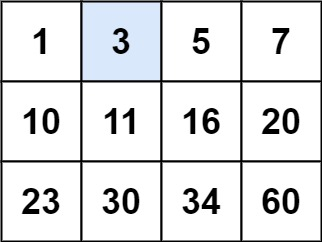
\includegraphics{d53fa452-c215-42f2-b450-86b22bc062d0.jpg}
\caption{mat.jpg}
\end{figure}

\begin{itemize}
\tightlist
\item
  Input: matrix =
  {[}{[}1,3,5,7{]},{[}10,11,16,20{]},{[}23,30,34,60{]}{]}, target = 13
\item
  Output: false
\end{itemize}

\begin{figure}
\centering
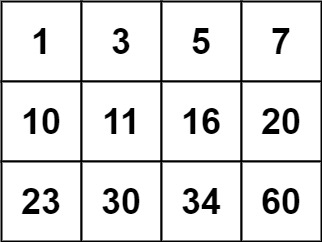
\includegraphics{fad32835-4ef4-4c98-84a5-ea52d4f3babd.jpg}
\caption{mat2.jpg}
\end{figure}

    \subsubsection{pseudocode}\label{pseudocode}

    \begin{tcolorbox}[breakable, size=fbox, boxrule=1pt, pad at break*=1mm,colback=cellbackground, colframe=cellborder]
\prompt{In}{incolor}{ }{\boxspacing}
\begin{Verbatim}[commandchars=\\\{\}]
\PY{n}{initialize} \PY{n}{m} \PY{o+ow}{and} \PY{n}{n} \PY{n}{to} \PY{n}{the} \PY{n}{number} \PY{n}{of} \PY{n}{rows} \PY{o+ow}{and} \PY{n}{columns} \PY{o+ow}{in} \PY{n}{the} \PY{n}{matrix}
\PY{n}{initialize} \PY{n}{left} \PY{n}{to} \PY{o}{\PYZhy{}}\PY{l+m+mi}{1} \PY{o+ow}{and} \PY{n}{right} \PY{n}{to} \PY{n}{the} \PY{n}{product} \PY{n}{of} \PY{n}{m} \PY{o+ow}{and} \PY{n}{n}
\PY{k}{while} \PY{n}{left} \PY{o}{+} \PY{l+m+mi}{1} \PY{o+ow}{is} \PY{n}{less} \PY{n}{than} \PY{n}{right}\PY{p}{:}
    \PY{n}{calculate} \PY{n}{mid} \PY{k}{as} \PY{n}{the} \PY{n}{average} \PY{n}{of} \PY{n}{left} \PY{o+ow}{and} \PY{n}{right}
    \PY{n+nb}{set} \PY{n}{x} \PY{n}{to} \PY{n}{the} \PY{n}{element} \PY{o+ow}{in} \PY{n}{the} \PY{n}{matrix} \PY{n}{at} \PY{n}{row} \PY{n}{mid} \PY{o}{/}\PY{o}{/} \PY{n}{n} \PY{o+ow}{and} \PY{n}{column} \PY{n}{mid} \PY{o}{\PYZpc{}} \PY{n}{n}
    \PY{k}{if} \PY{n}{x} \PY{o+ow}{is} \PY{n}{equal} \PY{n}{to} \PY{n}{target}\PY{p}{:}
        \PY{k}{return} \PY{n}{true}
    \PY{k}{if} \PY{n}{x} \PY{o+ow}{is} \PY{n}{less} \PY{n}{than} \PY{n}{target}\PY{p}{:}
        \PY{n+nb}{set} \PY{n}{left} \PY{n}{to} \PY{n}{mid}
    \PY{k}{else}\PY{p}{:}
        \PY{n+nb}{set} \PY{n}{right} \PY{n}{to} \PY{n}{mid}
\PY{k}{return} \PY{n}{false}
\end{Verbatim}
\end{tcolorbox}

    \subsubsection{Q74 code}\label{q74-code}

    \begin{tcolorbox}[breakable, size=fbox, boxrule=1pt, pad at break*=1mm,colback=cellbackground, colframe=cellborder]
\prompt{In}{incolor}{6}{\boxspacing}
\begin{Verbatim}[commandchars=\\\{\}]
\PY{k+kn}{from} \PY{n+nn}{typing} \PY{k+kn}{import} \PY{n}{List}

\PY{k}{class} \PY{n+nc}{Solution}\PY{p}{:}
    \PY{k}{def} \PY{n+nf}{searchMatrix}\PY{p}{(}\PY{n+nb+bp}{self}\PY{p}{,} \PY{n}{matrix}\PY{p}{:} \PY{n}{List}\PY{p}{[}\PY{n}{List}\PY{p}{[}\PY{n+nb}{int}\PY{p}{]}\PY{p}{]}\PY{p}{,} \PY{n}{target}\PY{p}{:} \PY{n+nb}{int}\PY{p}{)} \PY{o}{\PYZhy{}}\PY{o}{\PYZgt{}} \PY{n+nb}{bool}\PY{p}{:}
        \PY{n}{m}\PY{p}{,} \PY{n}{n} \PY{o}{=} \PY{n+nb}{len}\PY{p}{(}\PY{n}{matrix}\PY{p}{)}\PY{p}{,} \PY{n+nb}{len}\PY{p}{(}\PY{n}{matrix}\PY{p}{[}\PY{l+m+mi}{0}\PY{p}{]}\PY{p}{)}
        \PY{n}{left}\PY{p}{,} \PY{n}{right} \PY{o}{=} \PY{o}{\PYZhy{}}\PY{l+m+mi}{1}\PY{p}{,} \PY{n}{m} \PY{o}{*} \PY{n}{n}
        \PY{k}{while} \PY{n}{left} \PY{o}{+} \PY{l+m+mi}{1} \PY{o}{\PYZlt{}} \PY{n}{right}\PY{p}{:}
            \PY{n}{mid} \PY{o}{=} \PY{p}{(}\PY{n}{left} \PY{o}{+} \PY{n}{right}\PY{p}{)} \PY{o}{/}\PY{o}{/} \PY{l+m+mi}{2}
            \PY{n}{x} \PY{o}{=} \PY{n}{matrix}\PY{p}{[}\PY{n}{mid} \PY{o}{/}\PY{o}{/} \PY{n}{n}\PY{p}{]}\PY{p}{[}\PY{n}{mid} \PY{o}{\PYZpc{}} \PY{n}{n}\PY{p}{]}
            \PY{k}{if} \PY{n}{x} \PY{o}{==} \PY{n}{target}\PY{p}{:}
                \PY{k}{return} \PY{k+kc}{True}
            \PY{k}{if} \PY{n}{x} \PY{o}{\PYZlt{}} \PY{n}{target}\PY{p}{:}
                \PY{n}{left} \PY{o}{=} \PY{n}{mid}
            \PY{k}{else}\PY{p}{:}
                \PY{n}{right} \PY{o}{=} \PY{n}{mid}
        \PY{k}{return} \PY{k+kc}{False}

\PY{c+c1}{\PYZsh{} Test case}
\PY{n}{matrix} \PY{o}{=} \PY{p}{[}\PY{p}{[}\PY{l+m+mi}{1}\PY{p}{,} \PY{l+m+mi}{3}\PY{p}{,} \PY{l+m+mi}{5}\PY{p}{,} \PY{l+m+mi}{7}\PY{p}{]}\PY{p}{,} \PY{p}{[}\PY{l+m+mi}{10}\PY{p}{,} \PY{l+m+mi}{11}\PY{p}{,} \PY{l+m+mi}{16}\PY{p}{,} \PY{l+m+mi}{20}\PY{p}{]}\PY{p}{,} \PY{p}{[}\PY{l+m+mi}{23}\PY{p}{,} \PY{l+m+mi}{30}\PY{p}{,} \PY{l+m+mi}{34}\PY{p}{,} \PY{l+m+mi}{60}\PY{p}{]}\PY{p}{]}
\PY{n}{target} \PY{o}{=} \PY{l+m+mi}{3}
\PY{n}{solution} \PY{o}{=} \PY{n}{Solution}\PY{p}{(}\PY{p}{)}
\PY{n}{output} \PY{o}{=} \PY{n}{solution}\PY{o}{.}\PY{n}{searchMatrix}\PY{p}{(}\PY{n}{matrix}\PY{p}{,} \PY{n}{target}\PY{p}{)}
\PY{n+nb}{print}\PY{p}{(}\PY{l+s+sa}{f}\PY{l+s+s1}{\PYZsq{}}\PY{l+s+s1}{Input: matrix = }\PY{l+s+si}{\PYZob{}}\PY{n}{matrix}\PY{l+s+si}{\PYZcb{}}\PY{l+s+s1}{, target = }\PY{l+s+si}{\PYZob{}}\PY{n}{target}\PY{l+s+si}{\PYZcb{}}\PY{l+s+s1}{\PYZsq{}}\PY{p}{)}
\PY{n+nb}{print}\PY{p}{(}\PY{l+s+sa}{f}\PY{l+s+s1}{\PYZsq{}}\PY{l+s+s1}{Output: }\PY{l+s+si}{\PYZob{}}\PY{n}{output}\PY{l+s+si}{\PYZcb{}}\PY{l+s+s1}{\PYZsq{}}\PY{p}{)}
\end{Verbatim}
\end{tcolorbox}

    \begin{Verbatim}[commandchars=\\\{\}]
Input: matrix = [[1, 3, 5, 7], [10, 11, 16, 20], [23, 30, 34, 60]], target = 3
Output: True
    \end{Verbatim}

    Problem3-LeetcodeQ374. Guess Number Higher or Lower-Easy

We are playing the Guess Game. The game is as follows:

I pick a number from 1 to n.~You have to guess which number I picked.

Every time you guess wrong, I will tell you whether the number I picked
is higher or lower than your guess.

You call a pre-defined API int guess(int num), which returns three
possible results:

\begin{itemize}
\tightlist
\item
  -1: Your guess is higher than the number I picked (i.e.~num
  \textgreater{} pick).
\item
  1: Your guess is lower than the number I picked (i.e.~num \textless{}
  pick).
\item
  0: your guess is equal to the number I picked (i.e.~num == pick).
\item
  Return the number that I picked.
\end{itemize}

Example 1:

\begin{itemize}
\tightlist
\item
  Input: n = 10, pick = 6
\item
  Output: 6
\end{itemize}

Example 2:

\begin{itemize}
\tightlist
\item
  Input: n = 1, pick = 1
\item
  Output: 1
\end{itemize}

Example 3:

\begin{itemize}
\tightlist
\item
  Input: n = 2, pick = 1
\item
  Output: 1
\end{itemize}

    \subsubsection{pseudocode}\label{pseudocode}

    \begin{tcolorbox}[breakable, size=fbox, boxrule=1pt, pad at break*=1mm,colback=cellbackground, colframe=cellborder]
\prompt{In}{incolor}{ }{\boxspacing}
\begin{Verbatim}[commandchars=\\\{\}]
\PY{n}{initialize} \PY{n}{left} \PY{n}{to} \PY{l+m+mi}{1}
\PY{n}{initialize} \PY{n}{right} \PY{n}{to} \PY{n}{n}
\PY{k}{while} \PY{n}{left} \PY{o+ow}{is} \PY{n}{less} \PY{n}{than} \PY{o+ow}{or} \PY{n}{equal} \PY{n}{to} \PY{n}{right}\PY{p}{:}
\PY{n}{calculate} \PY{n}{mid} \PY{k}{as} \PY{n}{the} \PY{n}{average} \PY{n}{of} \PY{n}{left} \PY{o+ow}{and} \PY{n}{right}
\PY{n}{call} \PY{n}{the} \PY{n}{guess} \PY{n}{function} \PY{k}{with} \PY{n}{mid} \PY{o+ow}{and} \PY{n}{store} \PY{n}{the} \PY{n}{result} \PY{o+ow}{in} \PY{n}{ret}
\PY{k}{if} \PY{n}{ret} \PY{o+ow}{is} \PY{n}{equal} \PY{n}{to} \PY{l+m+mi}{0}\PY{p}{:}
    \PY{k}{return} \PY{n}{mid}
\PY{k}{if} \PY{n}{ret} \PY{o+ow}{is} \PY{n}{equal} \PY{n}{to} \PY{o}{\PYZhy{}}\PY{l+m+mi}{1}\PY{p}{:}
    \PY{n+nb}{set} \PY{n}{right} \PY{n}{to} \PY{n}{mid} \PY{o}{\PYZhy{}} \PY{l+m+mi}{1}
\PY{k}{else}\PY{p}{:}
    \PY{n+nb}{set} \PY{n}{left} \PY{n}{to} \PY{n}{mid} \PY{o}{+} \PY{l+m+mi}{1}
\end{Verbatim}
\end{tcolorbox}

    \subsubsection{code.py}\label{code.py}

    \begin{tcolorbox}[breakable, size=fbox, boxrule=1pt, pad at break*=1mm,colback=cellbackground, colframe=cellborder]
\prompt{In}{incolor}{8}{\boxspacing}
\begin{Verbatim}[commandchars=\\\{\}]
\PY{k}{def} \PY{n+nf}{guess}\PY{p}{(}\PY{n}{num}\PY{p}{:} \PY{n+nb}{int}\PY{p}{)} \PY{o}{\PYZhy{}}\PY{o}{\PYZgt{}} \PY{n+nb}{int}\PY{p}{:}
    \PY{n}{pick} \PY{o}{=} \PY{l+m+mi}{6} 
    \PY{k}{if} \PY{n}{num} \PY{o}{\PYZlt{}} \PY{n}{pick}\PY{p}{:}
        \PY{k}{return} \PY{l+m+mi}{1}
    \PY{k}{elif} \PY{n}{num} \PY{o}{\PYZgt{}} \PY{n}{pick}\PY{p}{:}
        \PY{k}{return} \PY{o}{\PYZhy{}}\PY{l+m+mi}{1}
    \PY{k}{else}\PY{p}{:}
        \PY{k}{return} \PY{l+m+mi}{0}

\PY{k+kn}{from} \PY{n+nn}{typing} \PY{k+kn}{import} \PY{n}{List}

\PY{k}{class} \PY{n+nc}{Solution}\PY{p}{:}
    \PY{k}{def} \PY{n+nf}{guessNumber}\PY{p}{(}\PY{n+nb+bp}{self}\PY{p}{,} \PY{n}{n}\PY{p}{:} \PY{n+nb}{int}\PY{p}{)} \PY{o}{\PYZhy{}}\PY{o}{\PYZgt{}} \PY{n+nb}{int}\PY{p}{:}
        \PY{n}{left} \PY{o}{=} \PY{l+m+mi}{1}
        \PY{n}{right} \PY{o}{=} \PY{n}{n}
        \PY{k}{while} \PY{n}{left} \PY{o}{\PYZlt{}}\PY{o}{=} \PY{n}{right}\PY{p}{:}
            \PY{n}{mid} \PY{o}{=} \PY{p}{(}\PY{n}{left} \PY{o}{+} \PY{n}{right}\PY{p}{)} \PY{o}{/}\PY{o}{/} \PY{l+m+mi}{2}
            \PY{n}{ret} \PY{o}{=} \PY{n}{guess}\PY{p}{(}\PY{n}{mid}\PY{p}{)}
            \PY{k}{if} \PY{n}{ret} \PY{o}{==} \PY{l+m+mi}{0}\PY{p}{:}
                \PY{k}{return} \PY{n}{mid}
            \PY{k}{elif} \PY{n}{ret} \PY{o}{==} \PY{o}{\PYZhy{}}\PY{l+m+mi}{1}\PY{p}{:}
                \PY{n}{right} \PY{o}{=} \PY{n}{mid} \PY{o}{\PYZhy{}} \PY{l+m+mi}{1}
            \PY{k}{else}\PY{p}{:}
                \PY{n}{left} \PY{o}{=} \PY{n}{mid} \PY{o}{+} \PY{l+m+mi}{1}

\PY{c+c1}{\PYZsh{} Test case}
\PY{n}{n} \PY{o}{=} \PY{l+m+mi}{10}
\PY{n}{solution} \PY{o}{=} \PY{n}{Solution}\PY{p}{(}\PY{p}{)}
\PY{n}{output} \PY{o}{=} \PY{n}{solution}\PY{o}{.}\PY{n}{guessNumber}\PY{p}{(}\PY{n}{n}\PY{p}{)}
\PY{n+nb}{print}\PY{p}{(}\PY{l+s+sa}{f}\PY{l+s+s1}{\PYZsq{}}\PY{l+s+s1}{Input: n = }\PY{l+s+si}{\PYZob{}}\PY{n}{n}\PY{l+s+si}{\PYZcb{}}\PY{l+s+s1}{, pick = 6}\PY{l+s+s1}{\PYZsq{}}\PY{p}{)}
\PY{n+nb}{print}\PY{p}{(}\PY{l+s+sa}{f}\PY{l+s+s1}{\PYZsq{}}\PY{l+s+s1}{Output: }\PY{l+s+si}{\PYZob{}}\PY{n}{output}\PY{l+s+si}{\PYZcb{}}\PY{l+s+s1}{\PYZsq{}}\PY{p}{)}
\end{Verbatim}
\end{tcolorbox}

    \begin{Verbatim}[commandchars=\\\{\}]
Input: n = 10, pick = 6
Output: 6
    \end{Verbatim}

    Problem4-LeetcodeQ278. First Bad Version-Easy

You are a product manager and currently leading a team to develop a new
product. Unfortunately, the latest version of your product fails the
quality check. Since each version is developed based on the previous
version, all the versions after a bad version are also bad.

Suppose you have n versions {[}1, 2, \ldots, n{]} and you want to find
out the first bad one, which causes all the following ones to be bad.

You are given an API bool isBadVersion(version) which returns whether
version is bad. Implement a function to find the first bad version. You
should minimize the number of calls to the API.

Example 1:

\begin{itemize}
\tightlist
\item
  Input: n = 5, bad = 4
\item
  Output: 4
\end{itemize}

Explanation: - call isBadVersion(3) -\textgreater{} false - call
isBadVersion(5) -\textgreater{} true - call isBadVersion(4)
-\textgreater{} true - Then 4 is the first bad version.

Example 2:

\begin{itemize}
\tightlist
\item
  Input: n = 1, bad = 1
\item
  Output: 1
\end{itemize}

    \subsubsection{pseudocode}\label{pseudocode}

    \begin{tcolorbox}[breakable, size=fbox, boxrule=1pt, pad at break*=1mm,colback=cellbackground, colframe=cellborder]
\prompt{In}{incolor}{ }{\boxspacing}
\begin{Verbatim}[commandchars=\\\{\}]
\PY{n}{initialize} \PY{n}{i} \PY{n}{to} \PY{l+m+mi}{1}
\PY{n}{initialize} \PY{n}{j} \PY{n}{to} \PY{n}{n}
\PY{k}{while} \PY{n}{i} \PY{o+ow}{is} \PY{n}{less} \PY{n}{than} \PY{o+ow}{or} \PY{n}{equal} \PY{n}{to} \PY{n}{j}\PY{p}{:}
\PY{n}{calculate} \PY{n}{m} \PY{k}{as} \PY{n}{the} \PY{n}{average} \PY{n}{of} \PY{n}{i} \PY{o+ow}{and} \PY{n}{j}
\PY{k}{if} \PY{n}{isBadVersion}\PY{p}{(}\PY{n}{m}\PY{p}{)} \PY{o+ow}{is} \PY{n}{true}\PY{p}{:}
    \PY{n+nb}{set} \PY{n}{j} \PY{n}{to} \PY{n}{m} \PY{o}{\PYZhy{}} \PY{l+m+mi}{1}
\PY{k}{else}\PY{p}{:}
    \PY{n+nb}{set} \PY{n}{i} \PY{n}{to} \PY{n}{m} \PY{o}{+} \PY{l+m+mi}{1}
\end{Verbatim}
\end{tcolorbox}

    \subsubsection{code.py}\label{code.py}

    \begin{tcolorbox}[breakable, size=fbox, boxrule=1pt, pad at break*=1mm,colback=cellbackground, colframe=cellborder]
\prompt{In}{incolor}{11}{\boxspacing}
\begin{Verbatim}[commandchars=\\\{\}]
\PY{k}{def} \PY{n+nf}{isBadVersion}\PY{p}{(}\PY{n}{version}\PY{p}{:} \PY{n+nb}{int}\PY{p}{)} \PY{o}{\PYZhy{}}\PY{o}{\PYZgt{}} \PY{n+nb}{bool}\PY{p}{:}
    \PY{n}{bad} \PY{o}{=} \PY{l+m+mi}{4}  \PY{c+c1}{\PYZsh{} example value for testing}
    \PY{k}{return} \PY{n}{version} \PY{o}{\PYZgt{}}\PY{o}{=} \PY{n}{bad}

\PY{k}{class} \PY{n+nc}{Solution}\PY{p}{:}
    \PY{k}{def} \PY{n+nf}{firstBadVersion}\PY{p}{(}\PY{n+nb+bp}{self}\PY{p}{,} \PY{n}{n}\PY{p}{:} \PY{n+nb}{int}\PY{p}{)} \PY{o}{\PYZhy{}}\PY{o}{\PYZgt{}} \PY{n+nb}{int}\PY{p}{:}
        \PY{n}{i}\PY{p}{,} \PY{n}{j} \PY{o}{=} \PY{l+m+mi}{1}\PY{p}{,} \PY{n}{n}
        \PY{k}{while} \PY{n}{i} \PY{o}{\PYZlt{}}\PY{o}{=} \PY{n}{j}\PY{p}{:}
            \PY{n}{m} \PY{o}{=} \PY{p}{(}\PY{n}{i} \PY{o}{+} \PY{n}{j}\PY{p}{)} \PY{o}{/}\PY{o}{/} \PY{l+m+mi}{2}
            \PY{k}{if} \PY{n}{isBadVersion}\PY{p}{(}\PY{n}{m}\PY{p}{)}\PY{p}{:}
                \PY{n}{j} \PY{o}{=} \PY{n}{m} \PY{o}{\PYZhy{}} \PY{l+m+mi}{1}
            \PY{k}{else}\PY{p}{:}
                \PY{n}{i} \PY{o}{=} \PY{n}{m} \PY{o}{+} \PY{l+m+mi}{1}
        \PY{k}{return} \PY{n}{i}

\PY{c+c1}{\PYZsh{} Test case}
\PY{n}{n} \PY{o}{=} \PY{l+m+mi}{5}
\PY{n}{solution} \PY{o}{=} \PY{n}{Solution}\PY{p}{(}\PY{p}{)}
\PY{n}{output} \PY{o}{=} \PY{n}{solution}\PY{o}{.}\PY{n}{firstBadVersion}\PY{p}{(}\PY{n}{n}\PY{p}{)}
\PY{n+nb}{print}\PY{p}{(}\PY{l+s+sa}{f}\PY{l+s+s1}{\PYZsq{}}\PY{l+s+s1}{Input: n = }\PY{l+s+si}{\PYZob{}}\PY{n}{n}\PY{l+s+si}{\PYZcb{}}\PY{l+s+s1}{, bad = 4}\PY{l+s+s1}{\PYZsq{}}\PY{p}{)}
\PY{n+nb}{print}\PY{p}{(}\PY{l+s+sa}{f}\PY{l+s+s1}{\PYZsq{}}\PY{l+s+s1}{Output: }\PY{l+s+si}{\PYZob{}}\PY{n}{output}\PY{l+s+si}{\PYZcb{}}\PY{l+s+s1}{\PYZsq{}}\PY{p}{)}
\end{Verbatim}
\end{tcolorbox}

    \begin{Verbatim}[commandchars=\\\{\}]
Input: n = 5, bad = 4
Output: 4
    \end{Verbatim}

    Problem5-LeetcodeQ875. Koko Eating Bananas-Medium

Koko loves to eat bananas. There are n piles of bananas, the ith pile
has piles{[}i{]} bananas. The guards have gone and will come back in h
hours.

Koko can decide her bananas-per-hour eating speed of k. Each hour, she
chooses some pile of bananas and eats k bananas from that pile. If the
pile has less than k bananas, she eats all of them instead and will not
eat any more bananas during this hour.

Koko likes to eat slowly but still wants to finish eating all the
bananas before the guards return.

Return the minimum integer k such that she can eat all the bananas
within h hours.

Example 1:

\begin{itemize}
\tightlist
\item
  Input: piles = {[}3,6,7,11{]}, h = 8
\item
  Output: 4
\end{itemize}

Example 2:

\begin{itemize}
\tightlist
\item
  Input: piles = {[}30,11,23,4,20{]}, h = 5
\item
  Output: 30
\end{itemize}

Example 3:

\begin{itemize}
\tightlist
\item
  Input: piles = {[}30,11,23,4,20{]}, h = 6
\item
  Output: 23
\end{itemize}

    \subsubsection{pseudocode}\label{pseudocode}

    \begin{tcolorbox}[breakable, size=fbox, boxrule=1pt, pad at break*=1mm,colback=cellbackground, colframe=cellborder]
\prompt{In}{incolor}{ }{\boxspacing}
\begin{Verbatim}[commandchars=\\\{\}]
\PY{n}{initialize} \PY{n}{n} \PY{n}{to} \PY{n}{the} \PY{n}{length} \PY{n}{of} \PY{n}{piles}
\PY{n}{initialize} \PY{n}{left} \PY{n}{to} \PY{l+m+mi}{0}
\PY{n}{initialize} \PY{n}{right} \PY{n}{to} \PY{n}{the} \PY{n}{maximum} \PY{n}{value} \PY{o+ow}{in} \PY{n}{piles}
\PY{k}{while} \PY{n}{left} \PY{o}{+} \PY{l+m+mi}{1} \PY{o+ow}{is} \PY{n}{less} \PY{n}{than} \PY{n}{right}\PY{p}{:}
    \PY{n}{calculate} \PY{n}{mid} \PY{k}{as} \PY{n}{the} \PY{n}{average} \PY{n}{of} \PY{n}{left} \PY{o+ow}{and} \PY{n}{right}
    \PY{k}{if} \PY{n}{the} \PY{n+nb}{sum} \PY{n}{of} \PY{p}{(}\PY{n}{p} \PY{o}{\PYZhy{}} \PY{l+m+mi}{1}\PY{p}{)} \PY{o}{/}\PY{o}{/} \PY{n}{mid} \PY{k}{for} \PY{n}{each} \PY{n}{p} \PY{o+ow}{in} \PY{n}{piles} \PY{o+ow}{is} \PY{n}{less} \PY{n}{than} \PY{o+ow}{or} \PY{n}{equal} \PY{n}{to} \PY{n}{h} \PY{o}{\PYZhy{}} \PY{n}{n}\PY{p}{:}
        \PY{n+nb}{set} \PY{n}{right} \PY{n}{to} \PY{n}{mid}
    \PY{k}{else}\PY{p}{:}
        \PY{n+nb}{set} \PY{n}{left} \PY{n}{to} \PY{n}{mid}
\PY{k}{return} \PY{n}{right}
\end{Verbatim}
\end{tcolorbox}

    \subsubsection{code.py}\label{code.py}

    \begin{tcolorbox}[breakable, size=fbox, boxrule=1pt, pad at break*=1mm,colback=cellbackground, colframe=cellborder]
\prompt{In}{incolor}{13}{\boxspacing}
\begin{Verbatim}[commandchars=\\\{\}]
\PY{k+kn}{from} \PY{n+nn}{typing} \PY{k+kn}{import} \PY{n}{List}

\PY{k}{class} \PY{n+nc}{Solution}\PY{p}{:}
    \PY{k}{def} \PY{n+nf}{minEatingSpeed}\PY{p}{(}\PY{n+nb+bp}{self}\PY{p}{,} \PY{n}{piles}\PY{p}{:} \PY{n}{List}\PY{p}{[}\PY{n+nb}{int}\PY{p}{]}\PY{p}{,} \PY{n}{h}\PY{p}{:} \PY{n+nb}{int}\PY{p}{)} \PY{o}{\PYZhy{}}\PY{o}{\PYZgt{}} \PY{n+nb}{int}\PY{p}{:}
        \PY{n}{n} \PY{o}{=} \PY{n+nb}{len}\PY{p}{(}\PY{n}{piles}\PY{p}{)}
        \PY{n}{left} \PY{o}{=} \PY{l+m+mi}{0}  
        \PY{n}{right} \PY{o}{=} \PY{n+nb}{max}\PY{p}{(}\PY{n}{piles}\PY{p}{)}  
        \PY{k}{while} \PY{n}{left} \PY{o}{+} \PY{l+m+mi}{1} \PY{o}{\PYZlt{}} \PY{n}{right}\PY{p}{:} 
            \PY{n}{mid} \PY{o}{=} \PY{p}{(}\PY{n}{left} \PY{o}{+} \PY{n}{right}\PY{p}{)} \PY{o}{/}\PY{o}{/} \PY{l+m+mi}{2}
            \PY{k}{if} \PY{n+nb}{sum}\PY{p}{(}\PY{p}{(}\PY{n}{p} \PY{o}{\PYZhy{}} \PY{l+m+mi}{1}\PY{p}{)} \PY{o}{/}\PY{o}{/} \PY{n}{mid} \PY{k}{for} \PY{n}{p} \PY{o+ow}{in} \PY{n}{piles}\PY{p}{)} \PY{o}{\PYZlt{}}\PY{o}{=} \PY{n}{h} \PY{o}{\PYZhy{}} \PY{n}{n}\PY{p}{:}
                \PY{n}{right} \PY{o}{=} \PY{n}{mid}  
            \PY{k}{else}\PY{p}{:}
                \PY{n}{left} \PY{o}{=} \PY{n}{mid} 
        \PY{k}{return} \PY{n}{right}  

\PY{c+c1}{\PYZsh{} Test case}
\PY{n}{piles} \PY{o}{=} \PY{p}{[}\PY{l+m+mi}{30}\PY{p}{,} \PY{l+m+mi}{11}\PY{p}{,} \PY{l+m+mi}{23}\PY{p}{,} \PY{l+m+mi}{4}\PY{p}{,} \PY{l+m+mi}{20}\PY{p}{]}
\PY{n}{h} \PY{o}{=} \PY{l+m+mi}{5}
\PY{n}{solution} \PY{o}{=} \PY{n}{Solution}\PY{p}{(}\PY{p}{)}
\PY{n}{output} \PY{o}{=} \PY{n}{solution}\PY{o}{.}\PY{n}{minEatingSpeed}\PY{p}{(}\PY{n}{piles}\PY{p}{,} \PY{n}{h}\PY{p}{)}
\PY{n+nb}{print}\PY{p}{(}\PY{l+s+sa}{f}\PY{l+s+s1}{\PYZsq{}}\PY{l+s+s1}{Input: piles = }\PY{l+s+si}{\PYZob{}}\PY{n}{piles}\PY{l+s+si}{\PYZcb{}}\PY{l+s+s1}{, h = }\PY{l+s+si}{\PYZob{}}\PY{n}{h}\PY{l+s+si}{\PYZcb{}}\PY{l+s+s1}{\PYZsq{}}\PY{p}{)}
\PY{n+nb}{print}\PY{p}{(}\PY{l+s+sa}{f}\PY{l+s+s1}{\PYZsq{}}\PY{l+s+s1}{Output: }\PY{l+s+si}{\PYZob{}}\PY{n}{output}\PY{l+s+si}{\PYZcb{}}\PY{l+s+s1}{\PYZsq{}}\PY{p}{)}
\end{Verbatim}
\end{tcolorbox}

    \begin{Verbatim}[commandchars=\\\{\}]
Input: piles = [30, 11, 23, 4, 20], h = 5
Output: 30
    \end{Verbatim}

    Problem6-LeetcodeQ700. Search in a Binary Search Tree-Easy

You are given the root of a binary search tree (BST) and an integer val.

Find the node in the BST that the node's value equals val and return the
subtree rooted with that node. If such a node does not exist, return
null.

Example1: - Input: root = {[}4,2,7,1,3{]}, val = 2 - Output: {[}2,1,3{]}
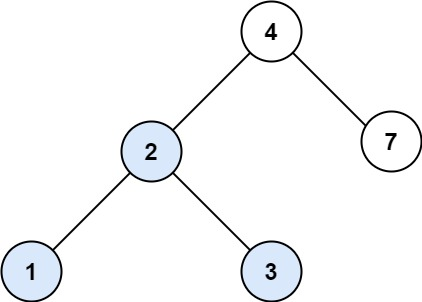
\includegraphics{af646e3b-a5bd-4985-9c3a-90586d7aa840.jpg}

Example2: - Input: root = {[}4,2,7,1,3{]}, val = 5 - Output: {[}{]}

\begin{figure}
\centering
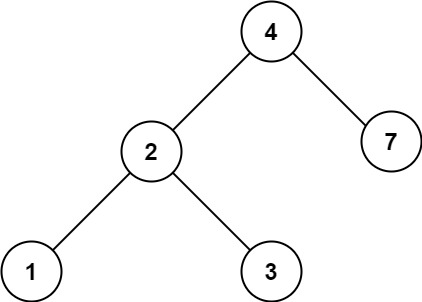
\includegraphics{9835ab4a-b937-44b0-9b2c-e293184f301e.jpg}
\caption{tree2.jpg}
\end{figure}

    \subsubsection{pseudocode}\label{pseudocode}

    \begin{tcolorbox}[breakable, size=fbox, boxrule=1pt, pad at break*=1mm,colback=cellbackground, colframe=cellborder]
\prompt{In}{incolor}{ }{\boxspacing}
\begin{Verbatim}[commandchars=\\\{\}]
\PY{k}{if} \PY{n}{root} \PY{o+ow}{is} \PY{n}{null}\PY{p}{:}
    \PY{k}{return} \PY{n}{null}
\PY{k}{else}\PY{p}{:}
    \PY{k}{if} \PY{n}{root} \PY{n}{value} \PY{o+ow}{is} \PY{n}{equal} \PY{n}{to} \PY{n}{val}\PY{p}{:}
        \PY{k}{return} \PY{n}{root}
    \PY{k}{else} \PY{k}{if} \PY{n}{root} \PY{n}{value} \PY{o+ow}{is} \PY{n}{greater} \PY{n}{than} \PY{n}{val}\PY{p}{:}
        \PY{k}{return} \PY{n}{searchBST} \PY{n}{on} \PY{n}{root}\PY{l+s+s1}{\PYZsq{}}\PY{l+s+s1}{s left child with val}
    \PY{k}{else}\PY{p}{:}
        \PY{k}{return} \PY{n}{searchBST} \PY{n}{on} \PY{n}{root}\PY{l+s+s1}{\PYZsq{}}\PY{l+s+s1}{s right child with val}
\PY{k}{return} \PY{n}{null}
\end{Verbatim}
\end{tcolorbox}

    \subsubsection{code.py}\label{code.py}

    \begin{tcolorbox}[breakable, size=fbox, boxrule=1pt, pad at break*=1mm,colback=cellbackground, colframe=cellborder]
\prompt{In}{incolor}{15}{\boxspacing}
\begin{Verbatim}[commandchars=\\\{\}]
\PY{k+kn}{from} \PY{n+nn}{typing} \PY{k+kn}{import} \PY{n}{Optional}

\PY{k}{class} \PY{n+nc}{TreeNode}\PY{p}{:}
    \PY{k}{def} \PY{n+nf+fm}{\PYZus{}\PYZus{}init\PYZus{}\PYZus{}}\PY{p}{(}\PY{n+nb+bp}{self}\PY{p}{,} \PY{n}{val}\PY{o}{=}\PY{l+m+mi}{0}\PY{p}{,} \PY{n}{left}\PY{o}{=}\PY{k+kc}{None}\PY{p}{,} \PY{n}{right}\PY{o}{=}\PY{k+kc}{None}\PY{p}{)}\PY{p}{:}
        \PY{n+nb+bp}{self}\PY{o}{.}\PY{n}{val} \PY{o}{=} \PY{n}{val}
        \PY{n+nb+bp}{self}\PY{o}{.}\PY{n}{left} \PY{o}{=} \PY{n}{left}
        \PY{n+nb+bp}{self}\PY{o}{.}\PY{n}{right} \PY{o}{=} \PY{n}{right}

\PY{k}{class} \PY{n+nc}{Solution}\PY{p}{:}
    \PY{k}{def} \PY{n+nf}{searchBST}\PY{p}{(}\PY{n+nb+bp}{self}\PY{p}{,} \PY{n}{root}\PY{p}{:} \PY{n}{Optional}\PY{p}{[}\PY{n}{TreeNode}\PY{p}{]}\PY{p}{,} \PY{n}{val}\PY{p}{:} \PY{n+nb}{int}\PY{p}{)} \PY{o}{\PYZhy{}}\PY{o}{\PYZgt{}} \PY{n}{Optional}\PY{p}{[}\PY{n}{TreeNode}\PY{p}{]}\PY{p}{:}
        \PY{k}{if} \PY{o+ow}{not} \PY{n}{root}\PY{p}{:}
            \PY{k}{return} \PY{k+kc}{None}
        \PY{k}{else}\PY{p}{:}
            \PY{k}{if} \PY{n}{root}\PY{o}{.}\PY{n}{val} \PY{o}{==} \PY{n}{val}\PY{p}{:}
                \PY{k}{return} \PY{n}{root}
            \PY{k}{elif} \PY{n}{root}\PY{o}{.}\PY{n}{val} \PY{o}{\PYZgt{}} \PY{n}{val}\PY{p}{:}
                \PY{k}{return} \PY{n+nb+bp}{self}\PY{o}{.}\PY{n}{searchBST}\PY{p}{(}\PY{n}{root}\PY{o}{.}\PY{n}{left}\PY{p}{,} \PY{n}{val}\PY{p}{)}
            \PY{k}{else}\PY{p}{:}
                \PY{k}{return} \PY{n+nb+bp}{self}\PY{o}{.}\PY{n}{searchBST}\PY{p}{(}\PY{n}{root}\PY{o}{.}\PY{n}{right}\PY{p}{,} \PY{n}{val}\PY{p}{)}
        \PY{k}{return} \PY{k+kc}{None}


\PY{k}{def} \PY{n+nf}{build\PYZus{}tree}\PY{p}{(}\PY{n}{nodes}\PY{p}{,} \PY{n}{index}\PY{o}{=}\PY{l+m+mi}{0}\PY{p}{)}\PY{p}{:}
    \PY{k}{if} \PY{n}{index} \PY{o}{\PYZlt{}} \PY{n+nb}{len}\PY{p}{(}\PY{n}{nodes}\PY{p}{)} \PY{o+ow}{and} \PY{n}{nodes}\PY{p}{[}\PY{n}{index}\PY{p}{]} \PY{o+ow}{is} \PY{o+ow}{not} \PY{k+kc}{None}\PY{p}{:}
        \PY{n}{node} \PY{o}{=} \PY{n}{TreeNode}\PY{p}{(}\PY{n}{nodes}\PY{p}{[}\PY{n}{index}\PY{p}{]}\PY{p}{)}
        \PY{n}{node}\PY{o}{.}\PY{n}{left} \PY{o}{=} \PY{n}{build\PYZus{}tree}\PY{p}{(}\PY{n}{nodes}\PY{p}{,} \PY{l+m+mi}{2} \PY{o}{*} \PY{n}{index} \PY{o}{+} \PY{l+m+mi}{1}\PY{p}{)}
        \PY{n}{node}\PY{o}{.}\PY{n}{right} \PY{o}{=} \PY{n}{build\PYZus{}tree}\PY{p}{(}\PY{n}{nodes}\PY{p}{,} \PY{l+m+mi}{2} \PY{o}{*} \PY{n}{index} \PY{o}{+} \PY{l+m+mi}{2}\PY{p}{)}
        \PY{k}{return} \PY{n}{node}
    \PY{k}{return} \PY{k+kc}{None}

\PY{k}{def} \PY{n+nf}{print\PYZus{}tree}\PY{p}{(}\PY{n}{node}\PY{p}{)}\PY{p}{:}
    \PY{k}{if} \PY{n}{node}\PY{p}{:}
        \PY{n}{print\PYZus{}tree}\PY{p}{(}\PY{n}{node}\PY{o}{.}\PY{n}{left}\PY{p}{)}
        \PY{n+nb}{print}\PY{p}{(}\PY{n}{node}\PY{o}{.}\PY{n}{val}\PY{p}{,} \PY{n}{end}\PY{o}{=}\PY{l+s+s1}{\PYZsq{}}\PY{l+s+s1}{ }\PY{l+s+s1}{\PYZsq{}}\PY{p}{)}
        \PY{n}{print\PYZus{}tree}\PY{p}{(}\PY{n}{node}\PY{o}{.}\PY{n}{right}\PY{p}{)}

\PY{c+c1}{\PYZsh{} Test case}
\PY{n}{root} \PY{o}{=} \PY{n}{build\PYZus{}tree}\PY{p}{(}\PY{p}{[}\PY{l+m+mi}{4}\PY{p}{,} \PY{l+m+mi}{2}\PY{p}{,} \PY{l+m+mi}{7}\PY{p}{,} \PY{l+m+mi}{1}\PY{p}{,} \PY{l+m+mi}{3}\PY{p}{]}\PY{p}{)}
\PY{n}{val} \PY{o}{=} \PY{l+m+mi}{2}
\PY{n}{solution} \PY{o}{=} \PY{n}{Solution}\PY{p}{(}\PY{p}{)}
\PY{n}{output} \PY{o}{=} \PY{n}{solution}\PY{o}{.}\PY{n}{searchBST}\PY{p}{(}\PY{n}{root}\PY{p}{,} \PY{n}{val}\PY{p}{)}
\PY{n+nb}{print}\PY{p}{(}\PY{l+s+sa}{f}\PY{l+s+s1}{\PYZsq{}}\PY{l+s+s1}{Input: root = [4, 2, 7, 1, 3], val = }\PY{l+s+si}{\PYZob{}}\PY{n}{val}\PY{l+s+si}{\PYZcb{}}\PY{l+s+s1}{\PYZsq{}}\PY{p}{)}
\PY{n+nb}{print}\PY{p}{(}\PY{l+s+sa}{f}\PY{l+s+s1}{\PYZsq{}}\PY{l+s+s1}{Output:}\PY{l+s+s1}{\PYZsq{}}\PY{p}{,} \PY{n}{end}\PY{o}{=}\PY{l+s+s1}{\PYZsq{}}\PY{l+s+s1}{ }\PY{l+s+s1}{\PYZsq{}}\PY{p}{)}
\PY{n}{print\PYZus{}tree}\PY{p}{(}\PY{n}{output}\PY{p}{)}
\PY{n+nb}{print}\PY{p}{(}\PY{p}{)}  
\end{Verbatim}
\end{tcolorbox}

    \begin{Verbatim}[commandchars=\\\{\}]
Input: root = [4, 2, 7, 1, 3], val = 2
Output: 1 2 3
    \end{Verbatim}

    Problem7-LeetcodeQ701. Insert into a Binary Search Tree-Medium

You are given the root node of a binary search tree (BST) and a value to
insert into the tree. Return the root node of the BST after the
insertion. It is guaranteed that the new value does not exist in the
original BST.

Notice that there may exist multiple valid ways for the insertion, as
long as the tree remains a BST after insertion. You can return any of
them.

Example1: - Input: root = {[}4,2,7,1,3{]}, val = 5 - Output:
{[}4,2,7,1,3,5{]}

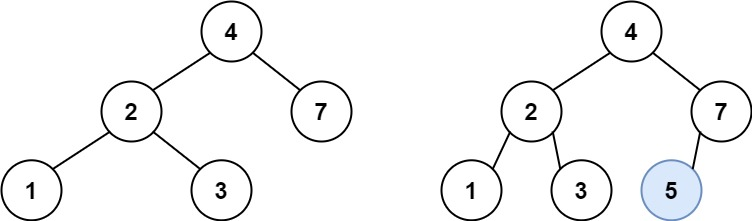
\includegraphics{8a906437-9735-41ed-8bc7-eece032e3c59.jpg}
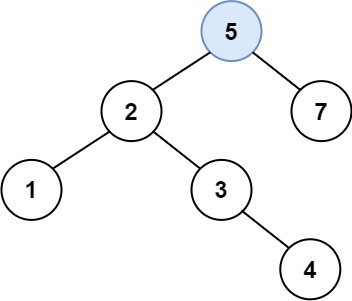
\includegraphics{41e872b4-fac2-4e4b-baa4-96e22c63a8b5.jpg}

Example 2:

\begin{itemize}
\tightlist
\item
  Input: root = {[}40,20,60,10,30,50,70{]}, val = 25
\item
  Output: {[}40,20,60,10,30,50,70,null,null,25{]}
\end{itemize}

Example 3:

\begin{itemize}
\tightlist
\item
  Input: root = {[}4,2,7,1,3,null,null,null,null,null,null{]}, val = 5
\item
  Output: {[}4,2,7,1,3,5{]}
\end{itemize}

    \subsubsection{pseudocode}\label{pseudocode}

    \begin{tcolorbox}[breakable, size=fbox, boxrule=1pt, pad at break*=1mm,colback=cellbackground, colframe=cellborder]
\prompt{In}{incolor}{ }{\boxspacing}
\begin{Verbatim}[commandchars=\\\{\}]
\PY{k}{if} \PY{n}{root} \PY{o+ow}{is} \PY{n}{null}\PY{p}{:}
\PY{k}{return} \PY{n}{new} \PY{n}{tree} \PY{n}{node} \PY{k}{with} \PY{n}{value} \PY{n}{val}

\PY{n}{define} \PY{n}{function} \PY{n}{find} \PY{k}{with} \PY{n}{parameters} \PY{n}{root}\PY{p}{,} \PY{n}{parent}\PY{p}{,} \PY{o+ow}{and} \PY{n}{val}\PY{p}{:}
\PY{k}{if} \PY{n}{root} \PY{o+ow}{is} \PY{n}{null}\PY{p}{:}
    \PY{k}{if} \PY{n}{val} \PY{o+ow}{is} \PY{n}{less} \PY{n}{than} \PY{n}{parent}\PY{l+s+s1}{\PYZsq{}}\PY{l+s+s1}{s value:}
    \PY{n+nb}{set} \PY{n}{parent}\PY{l+s+s1}{\PYZsq{}}\PY{l+s+s1}{s left child to new tree node with value val}
    \PY{k}{else}\PY{p}{:}
    \PY{n+nb}{set} \PY{n}{parent}\PY{l+s+s1}{\PYZsq{}}\PY{l+s+s1}{s right child to new tree node with value val}
    \PY{k}{return}
\PY{k}{if} \PY{n}{val} \PY{o+ow}{is} \PY{n}{less} \PY{n}{than} \PY{n}{root}\PY{l+s+s1}{\PYZsq{}}\PY{l+s+s1}{s value:}
    \PY{n}{call} \PY{n}{find} \PY{k}{with} \PY{n}{root}\PY{l+s+s1}{\PYZsq{}}\PY{l+s+s1}{s left child, root, and val}
\PY{k}{else}\PY{p}{:}
    \PY{n}{call} \PY{n}{find} \PY{k}{with} \PY{n}{root}\PY{l+s+s1}{\PYZsq{}}\PY{l+s+s1}{s right child, root, and val}

\PY{n}{call} \PY{n}{find} \PY{k}{with} \PY{n}{root}\PY{p}{,} \PY{n}{null}\PY{p}{,} \PY{o+ow}{and} \PY{n}{val}
\PY{k}{return} \PY{n}{root}
\end{Verbatim}
\end{tcolorbox}

    \subsubsection{code.py}\label{code.py}

    \begin{tcolorbox}[breakable, size=fbox, boxrule=1pt, pad at break*=1mm,colback=cellbackground, colframe=cellborder]
\prompt{In}{incolor}{17}{\boxspacing}
\begin{Verbatim}[commandchars=\\\{\}]
\PY{k+kn}{from} \PY{n+nn}{typing} \PY{k+kn}{import} \PY{n}{Optional}

\PY{k}{class} \PY{n+nc}{TreeNode}\PY{p}{:}
    \PY{k}{def} \PY{n+nf+fm}{\PYZus{}\PYZus{}init\PYZus{}\PYZus{}}\PY{p}{(}\PY{n+nb+bp}{self}\PY{p}{,} \PY{n}{val}\PY{o}{=}\PY{l+m+mi}{0}\PY{p}{,} \PY{n}{left}\PY{o}{=}\PY{k+kc}{None}\PY{p}{,} \PY{n}{right}\PY{o}{=}\PY{k+kc}{None}\PY{p}{)}\PY{p}{:}
        \PY{n+nb+bp}{self}\PY{o}{.}\PY{n}{val} \PY{o}{=} \PY{n}{val}
        \PY{n+nb+bp}{self}\PY{o}{.}\PY{n}{left} \PY{o}{=} \PY{n}{left}
        \PY{n+nb+bp}{self}\PY{o}{.}\PY{n}{right} \PY{o}{=} \PY{n}{right}

\PY{k}{class} \PY{n+nc}{Solution}\PY{p}{:}
    \PY{k}{def} \PY{n+nf}{insertIntoBST}\PY{p}{(}\PY{n+nb+bp}{self}\PY{p}{,} \PY{n}{root}\PY{p}{:} \PY{n}{Optional}\PY{p}{[}\PY{n}{TreeNode}\PY{p}{]}\PY{p}{,} \PY{n}{val}\PY{p}{:} \PY{n+nb}{int}\PY{p}{)} \PY{o}{\PYZhy{}}\PY{o}{\PYZgt{}} \PY{n}{TreeNode}\PY{p}{:}
        \PY{k}{if} \PY{n}{root} \PY{o+ow}{is} \PY{k+kc}{None}\PY{p}{:}
            \PY{k}{return} \PY{n}{TreeNode}\PY{p}{(}\PY{n}{val}\PY{p}{)}

        \PY{k}{def} \PY{n+nf}{find}\PY{p}{(}\PY{n}{root}\PY{p}{:} \PY{n}{Optional}\PY{p}{[}\PY{n}{TreeNode}\PY{p}{]}\PY{p}{,} \PY{n}{parent}\PY{p}{:} \PY{n}{Optional}\PY{p}{[}\PY{n}{TreeNode}\PY{p}{]}\PY{p}{,} \PY{n}{val}\PY{p}{:} \PY{n+nb}{int}\PY{p}{)}\PY{p}{:}
            \PY{k}{if} \PY{n}{root} \PY{o+ow}{is} \PY{k+kc}{None}\PY{p}{:}
                \PY{k}{if} \PY{n}{val} \PY{o}{\PYZlt{}} \PY{n}{parent}\PY{o}{.}\PY{n}{val}\PY{p}{:}
                    \PY{n}{parent}\PY{o}{.}\PY{n}{left} \PY{o}{=} \PY{n}{TreeNode}\PY{p}{(}\PY{n}{val}\PY{p}{)}
                \PY{k}{else}\PY{p}{:}
                    \PY{n}{parent}\PY{o}{.}\PY{n}{right} \PY{o}{=} \PY{n}{TreeNode}\PY{p}{(}\PY{n}{val}\PY{p}{)}
                \PY{k}{return}

            \PY{k}{if} \PY{n}{val} \PY{o}{\PYZlt{}} \PY{n}{root}\PY{o}{.}\PY{n}{val}\PY{p}{:}
                \PY{n}{find}\PY{p}{(}\PY{n}{root}\PY{o}{.}\PY{n}{left}\PY{p}{,} \PY{n}{root}\PY{p}{,} \PY{n}{val}\PY{p}{)}
            \PY{k}{else}\PY{p}{:}
                \PY{n}{find}\PY{p}{(}\PY{n}{root}\PY{o}{.}\PY{n}{right}\PY{p}{,} \PY{n}{root}\PY{p}{,} \PY{n}{val}\PY{p}{)}

        \PY{n}{find}\PY{p}{(}\PY{n}{root}\PY{p}{,} \PY{k+kc}{None}\PY{p}{,} \PY{n}{val}\PY{p}{)}
        \PY{k}{return} \PY{n}{root}

\PY{k}{def} \PY{n+nf}{build\PYZus{}tree}\PY{p}{(}\PY{n}{nodes}\PY{p}{,} \PY{n}{index}\PY{o}{=}\PY{l+m+mi}{0}\PY{p}{)}\PY{p}{:}
    \PY{k}{if} \PY{n}{index} \PY{o}{\PYZlt{}} \PY{n+nb}{len}\PY{p}{(}\PY{n}{nodes}\PY{p}{)} \PY{o+ow}{and} \PY{n}{nodes}\PY{p}{[}\PY{n}{index}\PY{p}{]} \PY{o+ow}{is} \PY{o+ow}{not} \PY{k+kc}{None}\PY{p}{:}
        \PY{n}{node} \PY{o}{=} \PY{n}{TreeNode}\PY{p}{(}\PY{n}{nodes}\PY{p}{[}\PY{n}{index}\PY{p}{]}\PY{p}{)}
        \PY{n}{node}\PY{o}{.}\PY{n}{left} \PY{o}{=} \PY{n}{build\PYZus{}tree}\PY{p}{(}\PY{n}{nodes}\PY{p}{,} \PY{l+m+mi}{2} \PY{o}{*} \PY{n}{index} \PY{o}{+} \PY{l+m+mi}{1}\PY{p}{)}
        \PY{n}{node}\PY{o}{.}\PY{n}{right} \PY{o}{=} \PY{n}{build\PYZus{}tree}\PY{p}{(}\PY{n}{nodes}\PY{p}{,} \PY{l+m+mi}{2} \PY{o}{*} \PY{n}{index} \PY{o}{+} \PY{l+m+mi}{2}\PY{p}{)}
        \PY{k}{return} \PY{n}{node}
    \PY{k}{return} \PY{k+kc}{None}

\PY{k}{def} \PY{n+nf}{print\PYZus{}tree}\PY{p}{(}\PY{n}{node}\PY{p}{)}\PY{p}{:}
    \PY{k}{if} \PY{n}{node}\PY{p}{:}
        \PY{n}{print\PYZus{}tree}\PY{p}{(}\PY{n}{node}\PY{o}{.}\PY{n}{left}\PY{p}{)}
        \PY{n+nb}{print}\PY{p}{(}\PY{n}{node}\PY{o}{.}\PY{n}{val}\PY{p}{,} \PY{n}{end}\PY{o}{=}\PY{l+s+s1}{\PYZsq{}}\PY{l+s+s1}{ }\PY{l+s+s1}{\PYZsq{}}\PY{p}{)}
        \PY{n}{print\PYZus{}tree}\PY{p}{(}\PY{n}{node}\PY{o}{.}\PY{n}{right}\PY{p}{)}

\PY{c+c1}{\PYZsh{} Test case}
\PY{n}{root} \PY{o}{=} \PY{n}{build\PYZus{}tree}\PY{p}{(}\PY{p}{[}\PY{l+m+mi}{4}\PY{p}{,} \PY{l+m+mi}{2}\PY{p}{,} \PY{l+m+mi}{7}\PY{p}{,} \PY{l+m+mi}{1}\PY{p}{,} \PY{l+m+mi}{3}\PY{p}{]}\PY{p}{)}
\PY{n}{val} \PY{o}{=} \PY{l+m+mi}{5}
\PY{n}{solution} \PY{o}{=} \PY{n}{Solution}\PY{p}{(}\PY{p}{)}
\PY{n}{output} \PY{o}{=} \PY{n}{solution}\PY{o}{.}\PY{n}{insertIntoBST}\PY{p}{(}\PY{n}{root}\PY{p}{,} \PY{n}{val}\PY{p}{)}
\PY{n+nb}{print}\PY{p}{(}\PY{l+s+sa}{f}\PY{l+s+s1}{\PYZsq{}}\PY{l+s+s1}{Input: root = [4, 2, 7, 1, 3], val = }\PY{l+s+si}{\PYZob{}}\PY{n}{val}\PY{l+s+si}{\PYZcb{}}\PY{l+s+s1}{\PYZsq{}}\PY{p}{)}
\PY{n+nb}{print}\PY{p}{(}\PY{l+s+sa}{f}\PY{l+s+s1}{\PYZsq{}}\PY{l+s+s1}{Output:}\PY{l+s+s1}{\PYZsq{}}\PY{p}{,} \PY{n}{end}\PY{o}{=}\PY{l+s+s1}{\PYZsq{}}\PY{l+s+s1}{ }\PY{l+s+s1}{\PYZsq{}}\PY{p}{)}
\PY{n}{print\PYZus{}tree}\PY{p}{(}\PY{n}{output}\PY{p}{)}
\PY{n+nb}{print}\PY{p}{(}\PY{p}{)} 
\end{Verbatim}
\end{tcolorbox}

    \begin{Verbatim}[commandchars=\\\{\}]
Input: root = [4, 2, 7, 1, 3], val = 5
Output: 1 2 3 4 5 7
    \end{Verbatim}

    Problem8-LeetcodeQ450. Delete Node in a BST-Medium

Given a root node reference of a BST and a key, delete the node with the
given key in the BST. Return the root node reference (possibly updated)
of the BST.

Basically, the deletion can be divided into two stages:

\begin{itemize}
\tightlist
\item
  Search for a node to remove.
\item
  If the node is found, delete the node.
\end{itemize}

Example 1:

\begin{figure}
\centering
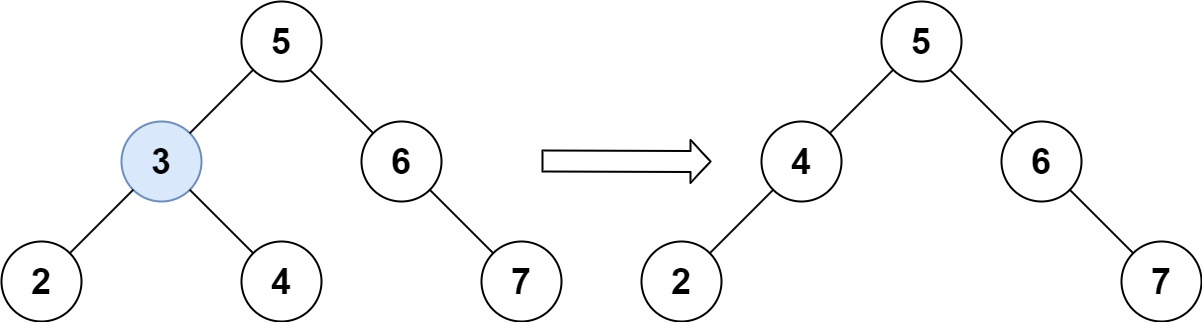
\includegraphics{fe13dfa1-1969-4a02-ba9e-ab0d0e828532.jpg}
\caption{del\_node\_1.jpg}
\end{figure}

\begin{itemize}
\tightlist
\item
  Input: root = {[}5,3,6,2,4,null,7{]}, key = 3
\item
  Output: {[}5,4,6,2,null,null,7{]}
\end{itemize}

Explanation: Given key to delete is 3. So we find the node with value 3
and delete it.

One valid answer is {[}5,4,6,2,null,null,7{]}, shown in the above BST.

Please notice that another valid answer is {[}5,2,6,null,4,null,7{]} and
it's also accepted.

Example 2:

\begin{figure}
\centering
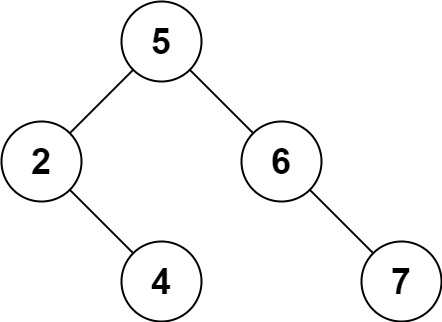
\includegraphics{7813d691-3f62-4e33-bee7-bb2a52c32015.jpg}
\caption{del\_node\_supp.jpg}
\end{figure}

\begin{itemize}
\tightlist
\item
  Input: root = {[}5,3,6,2,4,null,7{]}, key = 0
\item
  Output: {[}5,3,6,2,4,null,7{]}
\end{itemize}

Explanation: The tree does not contain a node with value = 0.

Example 3:

\begin{itemize}
\tightlist
\item
  Input: root = {[}{]}, key = 0
\item
  Output: {[}{]}
\end{itemize}

    \subsubsection{pseudocode}\label{pseudocode}

    \begin{tcolorbox}[breakable, size=fbox, boxrule=1pt, pad at break*=1mm,colback=cellbackground, colframe=cellborder]
\prompt{In}{incolor}{ }{\boxspacing}
\begin{Verbatim}[commandchars=\\\{\}]
\PY{k}{if} \PY{n}{root} \PY{o+ow}{is} \PY{o+ow}{not} \PY{n}{null}\PY{p}{:}
\PY{k}{if} \PY{n}{root} \PY{n}{value} \PY{o+ow}{is} \PY{n}{less} \PY{n}{than} \PY{n}{key}\PY{p}{:}
    \PY{n+nb}{set} \PY{n}{root}\PY{l+s+s1}{\PYZsq{}}\PY{l+s+s1}{s right child to the result of deleting the key from root}\PY{l+s+s1}{\PYZsq{}}\PY{n}{s} \PY{n}{right} \PY{n}{child}
\PY{k}{else} \PY{k}{if} \PY{n}{root} \PY{n}{value} \PY{o+ow}{is} \PY{n}{greater} \PY{n}{than} \PY{n}{key}\PY{p}{:}
    \PY{n+nb}{set} \PY{n}{root}\PY{l+s+s1}{\PYZsq{}}\PY{l+s+s1}{s left child to the result of deleting the key from root}\PY{l+s+s1}{\PYZsq{}}\PY{n}{s} \PY{n}{left} \PY{n}{child}
\PY{k}{else}\PY{p}{:}
    \PY{k}{if} \PY{n}{root} \PY{n}{has} \PY{n}{no} \PY{n}{left} \PY{o+ow}{or} \PY{n}{right} \PY{n}{child}\PY{p}{:}
        \PY{n+nb}{set} \PY{n}{root} \PY{n}{to} \PY{n}{root}\PY{l+s+s1}{\PYZsq{}}\PY{l+s+s1}{s left child if it exists, otherwise set to root}\PY{l+s+s1}{\PYZsq{}}\PY{n}{s} \PY{n}{right} \PY{n}{child}
    \PY{k}{else}\PY{p}{:}
        \PY{n}{initialize} \PY{n}{node} \PY{n}{to} \PY{n}{root}\PY{l+s+s1}{\PYZsq{}}\PY{l+s+s1}{s left child}
        \PY{k}{while} \PY{n}{node}\PY{l+s+s1}{\PYZsq{}}\PY{l+s+s1}{s right child exists:}
            \PY{n}{move} \PY{n}{to} \PY{n}{node}\PY{l+s+s1}{\PYZsq{}}\PY{l+s+s1}{s right child}
        \PY{n+nb}{set} \PY{n}{node}\PY{l+s+s1}{\PYZsq{}}\PY{l+s+s1}{s left child to the result of deleting node}\PY{l+s+s1}{\PYZsq{}}\PY{n}{s} \PY{n}{value} \PY{k+kn}{from} \PY{n+nn}{root}\PY{l+s+s1}{\PYZsq{}}\PY{l+s+s1}{s left child}
        \PY{n+nb}{set} \PY{n}{node}\PY{l+s+s1}{\PYZsq{}}\PY{l+s+s1}{s right child to root}\PY{l+s+s1}{\PYZsq{}}\PY{n}{s} \PY{n}{right} \PY{n}{child}
        \PY{n+nb}{set} \PY{n}{root} \PY{n}{to} \PY{n}{node}
\PY{k}{return} \PY{n}{root}
\end{Verbatim}
\end{tcolorbox}

    \subsubsection{code.py}\label{code.py}

    \begin{tcolorbox}[breakable, size=fbox, boxrule=1pt, pad at break*=1mm,colback=cellbackground, colframe=cellborder]
\prompt{In}{incolor}{20}{\boxspacing}
\begin{Verbatim}[commandchars=\\\{\}]
\PY{k+kn}{from} \PY{n+nn}{typing} \PY{k+kn}{import} \PY{n}{Optional}

\PY{k}{class} \PY{n+nc}{TreeNode}\PY{p}{:}
    \PY{k}{def} \PY{n+nf+fm}{\PYZus{}\PYZus{}init\PYZus{}\PYZus{}}\PY{p}{(}\PY{n+nb+bp}{self}\PY{p}{,} \PY{n}{val}\PY{o}{=}\PY{l+m+mi}{0}\PY{p}{,} \PY{n}{left}\PY{o}{=}\PY{k+kc}{None}\PY{p}{,} \PY{n}{right}\PY{o}{=}\PY{k+kc}{None}\PY{p}{)}\PY{p}{:}
        \PY{n+nb+bp}{self}\PY{o}{.}\PY{n}{val} \PY{o}{=} \PY{n}{val}
        \PY{n+nb+bp}{self}\PY{o}{.}\PY{n}{left} \PY{o}{=} \PY{n}{left}
        \PY{n+nb+bp}{self}\PY{o}{.}\PY{n}{right} \PY{o}{=} \PY{n}{right}

\PY{k}{class} \PY{n+nc}{Solution}\PY{p}{:}
    \PY{k}{def} \PY{n+nf}{deleteNode}\PY{p}{(}\PY{n+nb+bp}{self}\PY{p}{,} \PY{n}{root}\PY{p}{:} \PY{n}{Optional}\PY{p}{[}\PY{n}{TreeNode}\PY{p}{]}\PY{p}{,} \PY{n}{key}\PY{p}{:} \PY{n+nb}{int}\PY{p}{)} \PY{o}{\PYZhy{}}\PY{o}{\PYZgt{}} \PY{n}{Optional}\PY{p}{[}\PY{n}{TreeNode}\PY{p}{]}\PY{p}{:}
        \PY{k}{if} \PY{n}{root}\PY{p}{:}
            \PY{k}{if} \PY{n}{root}\PY{o}{.}\PY{n}{val} \PY{o}{\PYZlt{}} \PY{n}{key}\PY{p}{:}
                \PY{n}{root}\PY{o}{.}\PY{n}{right} \PY{o}{=} \PY{n+nb+bp}{self}\PY{o}{.}\PY{n}{deleteNode}\PY{p}{(}\PY{n}{root}\PY{o}{.}\PY{n}{right}\PY{p}{,} \PY{n}{key}\PY{p}{)}
            \PY{k}{elif} \PY{n}{root}\PY{o}{.}\PY{n}{val} \PY{o}{\PYZgt{}} \PY{n}{key}\PY{p}{:}
                \PY{n}{root}\PY{o}{.}\PY{n}{left} \PY{o}{=} \PY{n+nb+bp}{self}\PY{o}{.}\PY{n}{deleteNode}\PY{p}{(}\PY{n}{root}\PY{o}{.}\PY{n}{left}\PY{p}{,} \PY{n}{key}\PY{p}{)}
            \PY{k}{else}\PY{p}{:}
                \PY{k}{if} \PY{o+ow}{not} \PY{n}{root}\PY{o}{.}\PY{n}{left} \PY{o+ow}{or} \PY{o+ow}{not} \PY{n}{root}\PY{o}{.}\PY{n}{right}\PY{p}{:}
                    \PY{n}{root} \PY{o}{=} \PY{n}{root}\PY{o}{.}\PY{n}{left} \PY{k}{if} \PY{n}{root}\PY{o}{.}\PY{n}{left} \PY{k}{else} \PY{n}{root}\PY{o}{.}\PY{n}{right}
                \PY{k}{else}\PY{p}{:}
                    \PY{n}{node} \PY{o}{=} \PY{n}{root}\PY{o}{.}\PY{n}{left}
                    \PY{k}{while} \PY{n}{node}\PY{o}{.}\PY{n}{right}\PY{p}{:}
                        \PY{n}{node} \PY{o}{=} \PY{n}{node}\PY{o}{.}\PY{n}{right}
                    \PY{n}{node}\PY{o}{.}\PY{n}{left} \PY{o}{=} \PY{n+nb+bp}{self}\PY{o}{.}\PY{n}{deleteNode}\PY{p}{(}\PY{n}{root}\PY{o}{.}\PY{n}{left}\PY{p}{,} \PY{n}{node}\PY{o}{.}\PY{n}{val}\PY{p}{)}
                    \PY{n}{node}\PY{o}{.}\PY{n}{right} \PY{o}{=} \PY{n}{root}\PY{o}{.}\PY{n}{right}
                    \PY{n}{root} \PY{o}{=} \PY{n}{node}
        \PY{k}{return} \PY{n}{root}


\PY{k}{def} \PY{n+nf}{build\PYZus{}tree}\PY{p}{(}\PY{n}{nodes}\PY{p}{,} \PY{n}{index}\PY{o}{=}\PY{l+m+mi}{0}\PY{p}{)}\PY{p}{:}
    \PY{k}{if} \PY{n}{index} \PY{o}{\PYZlt{}} \PY{n+nb}{len}\PY{p}{(}\PY{n}{nodes}\PY{p}{)} \PY{o+ow}{and} \PY{n}{nodes}\PY{p}{[}\PY{n}{index}\PY{p}{]} \PY{o+ow}{is} \PY{o+ow}{not} \PY{k+kc}{None}\PY{p}{:}
        \PY{n}{node} \PY{o}{=} \PY{n}{TreeNode}\PY{p}{(}\PY{n}{nodes}\PY{p}{[}\PY{n}{index}\PY{p}{]}\PY{p}{)}
        \PY{n}{node}\PY{o}{.}\PY{n}{left} \PY{o}{=} \PY{n}{build\PYZus{}tree}\PY{p}{(}\PY{n}{nodes}\PY{p}{,} \PY{l+m+mi}{2} \PY{o}{*} \PY{n}{index} \PY{o}{+} \PY{l+m+mi}{1}\PY{p}{)}
        \PY{n}{node}\PY{o}{.}\PY{n}{right} \PY{o}{=} \PY{n}{build\PYZus{}tree}\PY{p}{(}\PY{n}{nodes}\PY{p}{,} \PY{l+m+mi}{2} \PY{o}{*} \PY{n}{index} \PY{o}{+} \PY{l+m+mi}{2}\PY{p}{)}
        \PY{k}{return} \PY{n}{node}
    \PY{k}{return} \PY{k+kc}{None}

\PY{k}{def} \PY{n+nf}{print\PYZus{}tree}\PY{p}{(}\PY{n}{node}\PY{p}{)}\PY{p}{:}
    \PY{k}{if} \PY{n}{node}\PY{p}{:}
        \PY{n}{print\PYZus{}tree}\PY{p}{(}\PY{n}{node}\PY{o}{.}\PY{n}{left}\PY{p}{)}
        \PY{n+nb}{print}\PY{p}{(}\PY{n}{node}\PY{o}{.}\PY{n}{val}\PY{p}{,} \PY{n}{end}\PY{o}{=}\PY{l+s+s1}{\PYZsq{}}\PY{l+s+s1}{ }\PY{l+s+s1}{\PYZsq{}}\PY{p}{)}
        \PY{n}{print\PYZus{}tree}\PY{p}{(}\PY{n}{node}\PY{o}{.}\PY{n}{right}\PY{p}{)}

\PY{c+c1}{\PYZsh{} Test case}
\PY{n}{root} \PY{o}{=} \PY{n}{build\PYZus{}tree}\PY{p}{(}\PY{p}{[}\PY{l+m+mi}{5}\PY{p}{,} \PY{l+m+mi}{3}\PY{p}{,} \PY{l+m+mi}{6}\PY{p}{,} \PY{l+m+mi}{2}\PY{p}{,} \PY{l+m+mi}{4}\PY{p}{,} \PY{k+kc}{None}\PY{p}{,} \PY{l+m+mi}{7}\PY{p}{]}\PY{p}{)}
\PY{n}{key} \PY{o}{=} \PY{l+m+mi}{3}
\PY{n}{solution} \PY{o}{=} \PY{n}{Solution}\PY{p}{(}\PY{p}{)}
\PY{n}{output} \PY{o}{=} \PY{n}{solution}\PY{o}{.}\PY{n}{deleteNode}\PY{p}{(}\PY{n}{root}\PY{p}{,} \PY{n}{key}\PY{p}{)}
\PY{n+nb}{print}\PY{p}{(}\PY{l+s+sa}{f}\PY{l+s+s1}{\PYZsq{}}\PY{l+s+s1}{Input: root = [5, 3, 6, 2, 4, null, 7], key = }\PY{l+s+si}{\PYZob{}}\PY{n}{key}\PY{l+s+si}{\PYZcb{}}\PY{l+s+s1}{\PYZsq{}}\PY{p}{)}
\PY{n+nb}{print}\PY{p}{(}\PY{l+s+sa}{f}\PY{l+s+s1}{\PYZsq{}}\PY{l+s+s1}{Output:}\PY{l+s+s1}{\PYZsq{}}\PY{p}{,} \PY{n}{end}\PY{o}{=}\PY{l+s+s1}{\PYZsq{}}\PY{l+s+s1}{ }\PY{l+s+s1}{\PYZsq{}}\PY{p}{)}
\PY{n}{print\PYZus{}tree}\PY{p}{(}\PY{n}{output}\PY{p}{)}
\PY{n+nb}{print}\PY{p}{(}\PY{p}{)} 
\end{Verbatim}
\end{tcolorbox}

    \begin{Verbatim}[commandchars=\\\{\}]
Input: root = [5, 3, 6, 2, 4, null, 7], key = 3
Output: 2 4 5 6 7
    \end{Verbatim}

    \begin{tcolorbox}[breakable, size=fbox, boxrule=1pt, pad at break*=1mm,colback=cellbackground, colframe=cellborder]
\prompt{In}{incolor}{ }{\boxspacing}
\begin{Verbatim}[commandchars=\\\{\}]

\end{Verbatim}
\end{tcolorbox}


    % Add a bibliography block to the postdoc
    
    
    
\end{document}
